%%%%%%%%%%%%%%%%%%%%%%%%%%%%%%%%%%%%%%%%%
% Journal Article
% LaTeX Template
% Version 1.4 (15/5/16)
%
% This template has been downloaded from:
% http://www.LaTeXTemplates.com
%
% Original author:
% Frits Wenneker (http://www.howtotex.com) with extensive modifications by
% Vel (vel@LaTeXTemplates.com)
%
% License:
% CC BY-NC-SA 3.0 (http://creativecommons.org/licenses/by-nc-sa/3.0/)
%
%%%%%%%%%%%%%%%%%%%%%%%%%%%%%%%%%%%%%%%%%

%----------------------------------------------------------------------------------------
%	PACKAGES AND OTHER DOCUMENT CONFIGURATIONS
%----------------------------------------------------------------------------------------

\documentclass{article}

\usepackage{blindtext} % Package to generate dummy text throughout this template 
\usepackage{indentfirst}
\usepackage[sc]{mathpazo} % Use the Palatino font
\usepackage[T1]{fontenc} % Use 8-bit encoding that has 256 glyphs
\linespread{1.05} % Line spacing - Palatino needs more space between lines
\usepackage{microtype} % Slightly tweak font spacing for aesthetics
\usepackage{graphicx}
\usepackage[english]{babel} % Language hyphenation and typographical rules
\usepackage{float}
\usepackage[hmarginratio=1:1,top=32mm,columnsep=20pt]{geometry} % Document margins
\usepackage[hang, small,labelfont=bf,up,textfont=it,up]{caption} % Custom captions under/above floats in tables or figures
\usepackage{booktabs} % Horizontal rules in tables

\usepackage{lettrine} % The lettrine is the first enlarged letter at the beginning of the text

\usepackage{enumitem} % Customized lists
\setlist[itemize]{noitemsep} % Make itemize lists more compact

\usepackage{abstract} % Allows abstract customization
\renewcommand{\abstractnamefont}{\normalfont\bfseries} % Set the "Abstract" text to bold
\renewcommand{\abstracttextfont}{\normalfont\small\itshape} % Set the abstract itself to small italic text

\usepackage{titlesec} % Allows customization of titles
\renewcommand\thesection{\roman{section}} % Roman numerals for the sections
\renewcommand{\thesubsection}{\thesection\alph{subsection}}
\titleformat{\section}[block]{\LARGE\scshape}{\thesection.}{1em}{} % Change the look of the section titles
\titleformat{\subsection}[block]{\large\scshape}{\thesubsection.}{1em}{} % Change the look of the section titles
\renewcommand{\thesubsubsection}{\thesection.\thesubsection.\alph{subsubsection}}
\titleformat{\subsubsection}[block]{\small\scshape}{\thesubsubsection.}{1em}{}
\usepackage{fancyhdr} % Headers and footers
\pagestyle{fancy} % All pages have headers and footers
\fancyhead{} % Blank out the default header
\fancyfoot{} % Blank out the default footer

\fancyfoot[RO,LE]{\thepage} % Custom footer text

\usepackage{titling} % Customizing the title section

\usepackage{hyperref} % For hyperlinks in the PDF

%----------------------------------------------------------------------------------------
%	TITLE SECTION
%----------------------------------------------------------------------------------------
\setlength{\parskip}{1em}
\setlength{\droptitle}{-7\baselineskip} % Move the title up

%\pretitle{\begin{center}% Article title formatting
%\posttitle{\end{center}} % Article title closing formatting
\title{\textbf{East Coast Regional Datathon 2021}} % Article title
\author{Team 24}
\date{March 2021} 



%----------------------------------------------------------------------------------------

\begin{document}

% Print the title
\maketitle

%----------------------------------------------------------------------------------------
%	ARTICLE CONTENTS
%----------------------------------------------------------------------------------------

\section{Executive Summary}
\subsection{Problem Statement}
In the years 2009-2012, Futbol Club Barcelona (Spain) came up with a unique strategy widely known as "Tiki-Taka"\cite{1}. In this style of play, the entire team comes together in a cluster and maintain control of the ball in that cluster\cite{2}. Following the Tiki-Taka strategy, Barcelona won 14 titles from 2008 to 2014. However, other club managers quickly devised counter-strategies to Tiki-Taka. These counter-strategies were so effective against Tiki-Taka that it practically died soon after 2012\cite{3}. 

There does not exist a universal strategy that will always win the game. We expect, however, like most strategy games, there exist an assortment of viable strategies, each with its own winning and losing match-ups. As such, question we seek to answer is: do European football teams develop multiple meta-game strategies (metas)? If so, how do different metas interact with each other and how can we use these winning relationships to find the best strategy against a specific opponent?

\subsection{Key Findings}
In this report, we present a \emph{metagame analysis} on European football games between 2008-2016. Through clustering algorithms, we show there are indeed meta-game interactions between team strategies, each with its own winning and losing match-ups. From these clusters, we also identified various prominent features that could explain some of the match-up breakdown. 
\par On the other hand, we have also identified one clusters as an anomaly as it is primarily defined by high overall ratings of players. This seem to suggest that the individual proficiency of players might be enough to offset strategic disadvantages in soccer. Furthermore, we were unable to identify `cycles' of meta-strategies that dominate one another, but instead found multiple `chains' of dominance. This seems to suggest that while there are meta-strategies in European football, other practical limitations in the game might make it difficult to see the full evolution of a game meta. In particular, we postulate that player contracts and inflexibility of teams in adopting new play styles could contribute to the lack of a fully developed metagame in European soccer.
\par Last but not least, using this meta-strategy table, we present a suggestion of counter strategies to adopt against other teams. Through a hypothesis testing procedure, we were able to reject the null hypothesis that ``the best counter meta recommended by us does not increase the expected number of goals''. 

\section{Technical Exposition}

\subsection{Data and Measures}
To minimize the effect of noise, our main goal in the data wrangling process is to create and identify all relevant attributes that could distinguish a particular meta-strategy from others. 
\begin{figure}[H]
\centering
    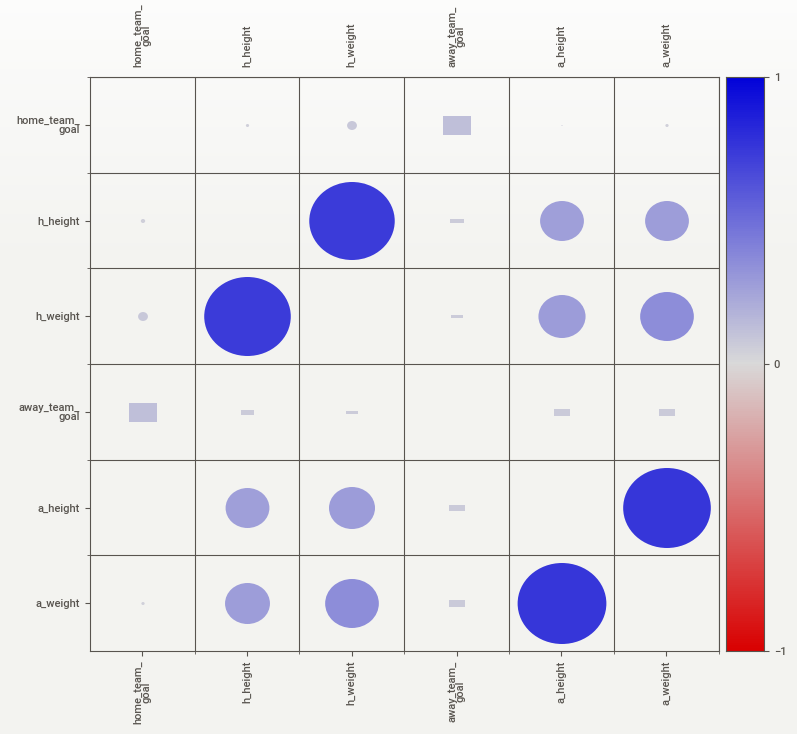
\includegraphics[width=.6\textwidth]{htwt_vs_goals.png}
    \caption{Correlation between height/weight information and home/away team goals}
\end{figure}
\par We attempted this by extending `match.csv' with the team attributes as well as the aggregated player attributes for each team. The reason for including individual player attributes is so that we can contextualize the team attributes. For instance, we might expect a strategy of sending long balls to star strikers in the center and one of sending through balls to wing players to both have similar team attributes, but might have distinct breakdown in terms of preferred foot of players. 

\par We have also made a decision to include the average player height and weight information for each team. While the dataset showed little correlation between the average height/weight and the goals scored, we identified that there is a possibility that height/weight information is only important in identifying particular meta-strategies but not goals scored in general. After all, it is well-known the advantages that height and build can bring to challenging the opposition in headers, possessions, and \emph{set pieces} \footnote{A set piece refers to a play scenario when the ball is out of bounds, including corner kicks, free kicks and penalties}. We later found this to be an accurate assessment, as our some of the identified meta-strategies include height and weight attributes in its classifying decision tree. 
\par Discrete attributes deserved their own unique treatments. We had to remove noisy discrete labels such as `y' and `stoc' under the `attacking work rate' attribute. Upon reviewing the source of the data, we realized that there are only 3 true labels for this attribute, namely `low', `medium' and `high'. Noisy labels are likely due to conversion errors from labels of other attributes such as the `stocky' label under `build' attribute which was excluded in the given dataset. 

\subsection{Preliminary Analysis}
Our goal in the preliminary analysis is to see if our assumption on football metagames is valid. To this end, we run a simple K-means clustering algorithm on team-wide features that are processed from team{\_}attributes.csv. We notice that many categorical columns in the data set are redundant information. Therefore, we take all numeric columns in team attributes to be features for K-means.

We normalize features by performing linear transformations on each feature so that the minimum and maximum values are transformed to 0 and 1, respectively. We choose min-max normalization over other normalization methods such as Normal standardization because the given data follow various unimodal distributions with similar minimum and maximum boundaries, as shown in Figure \ref{fig:k-means}. Meanwhile, there are no outliers after our data cleaning process. This suggests robust scaling does not offer significant advantage either.

\begin{figure}[H]
\centering
\begin{tabular}{ccc}
  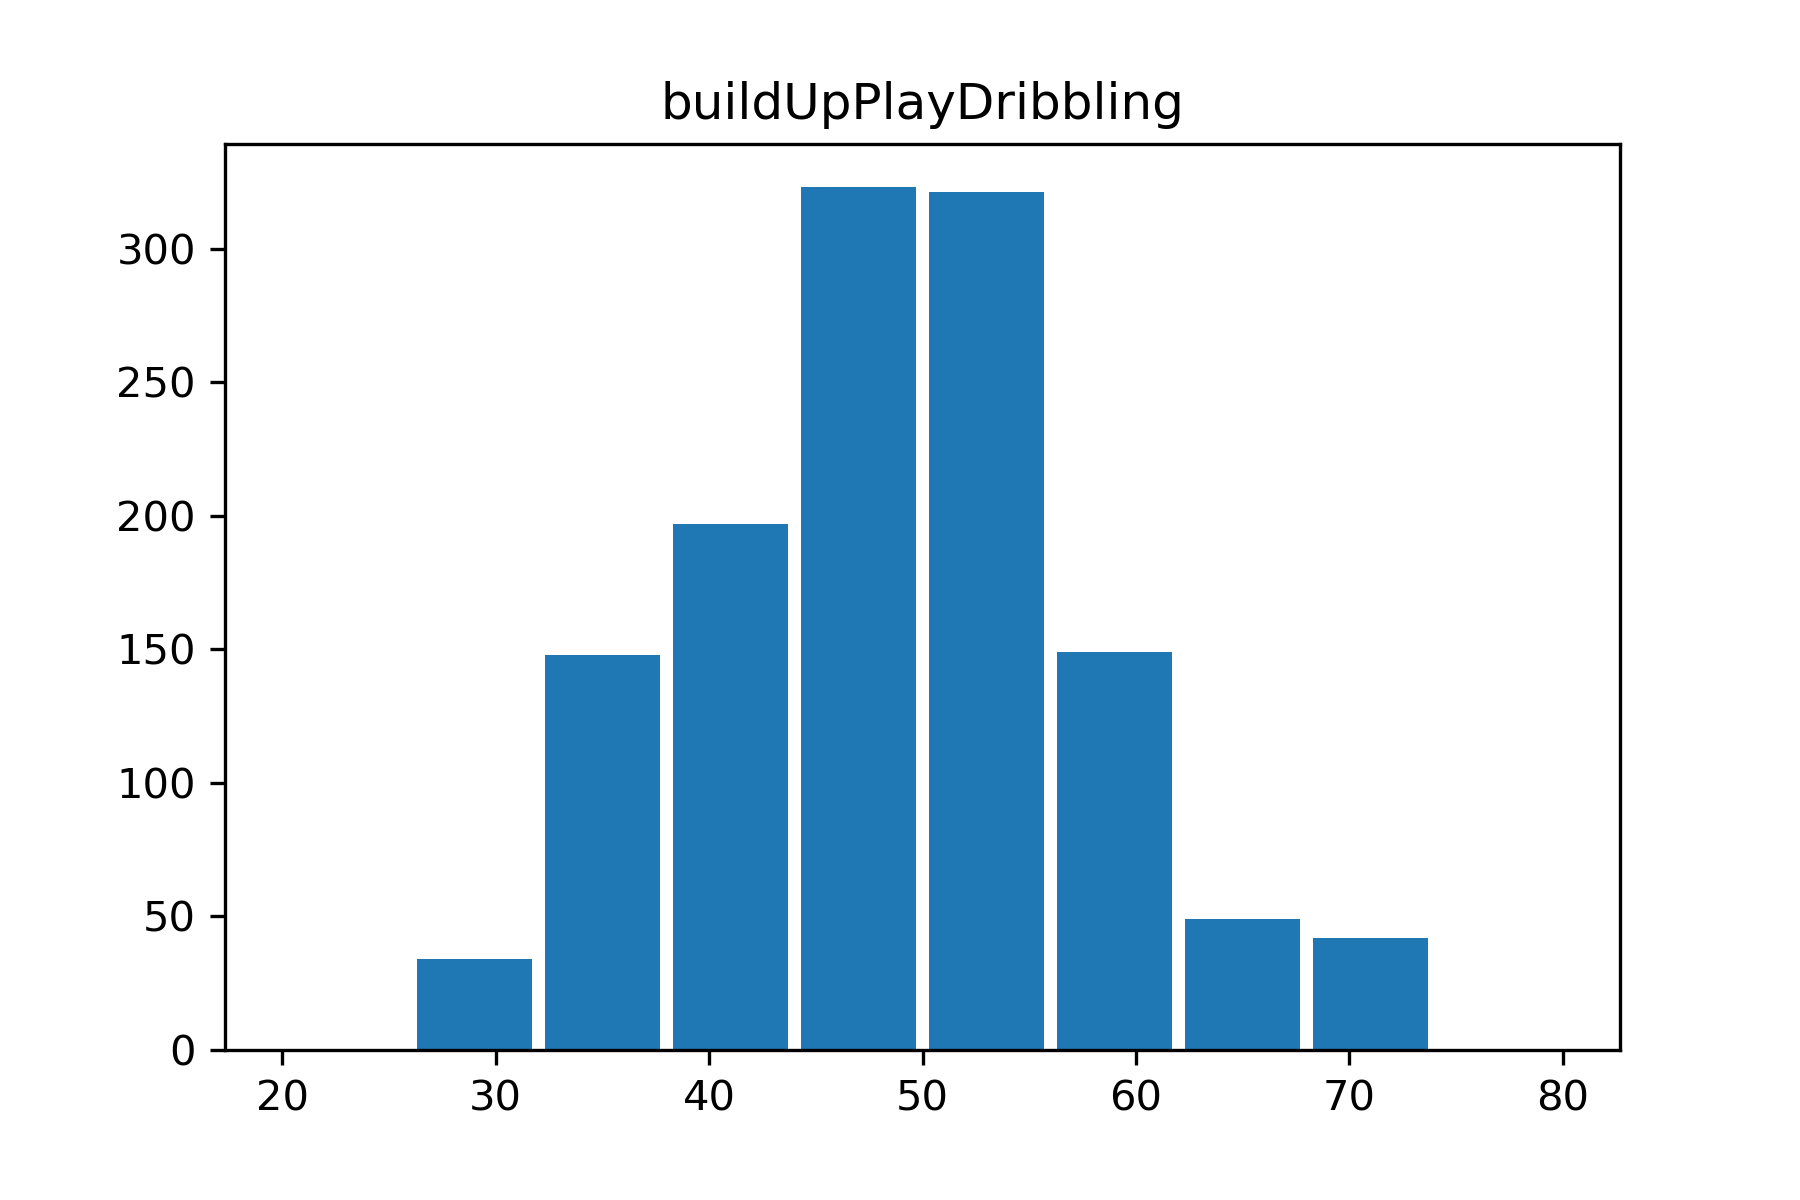
\includegraphics[width=40mm]{k-means_graphs/buildUpPlayDribbling.png} &   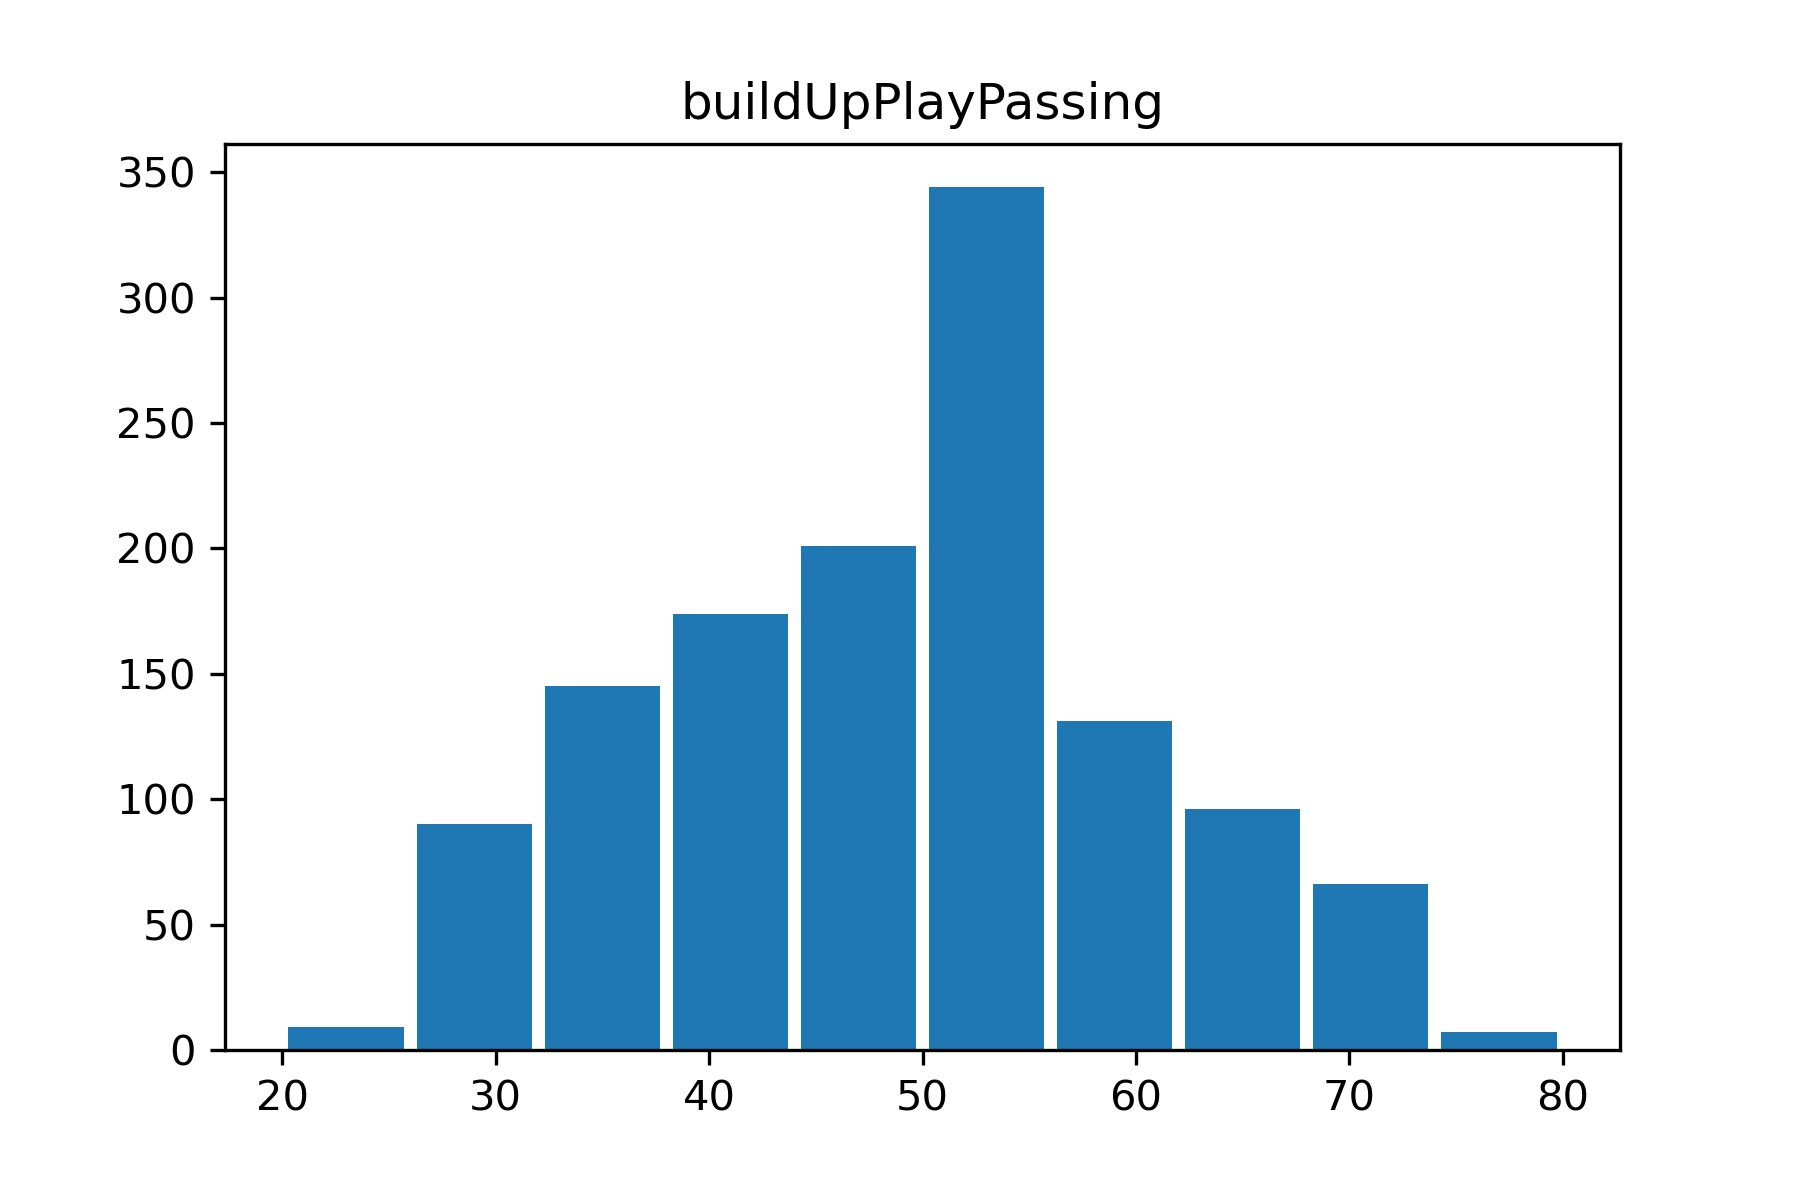
\includegraphics[width=40mm]{k-means_graphs/buildUpPlayPassing.png} &   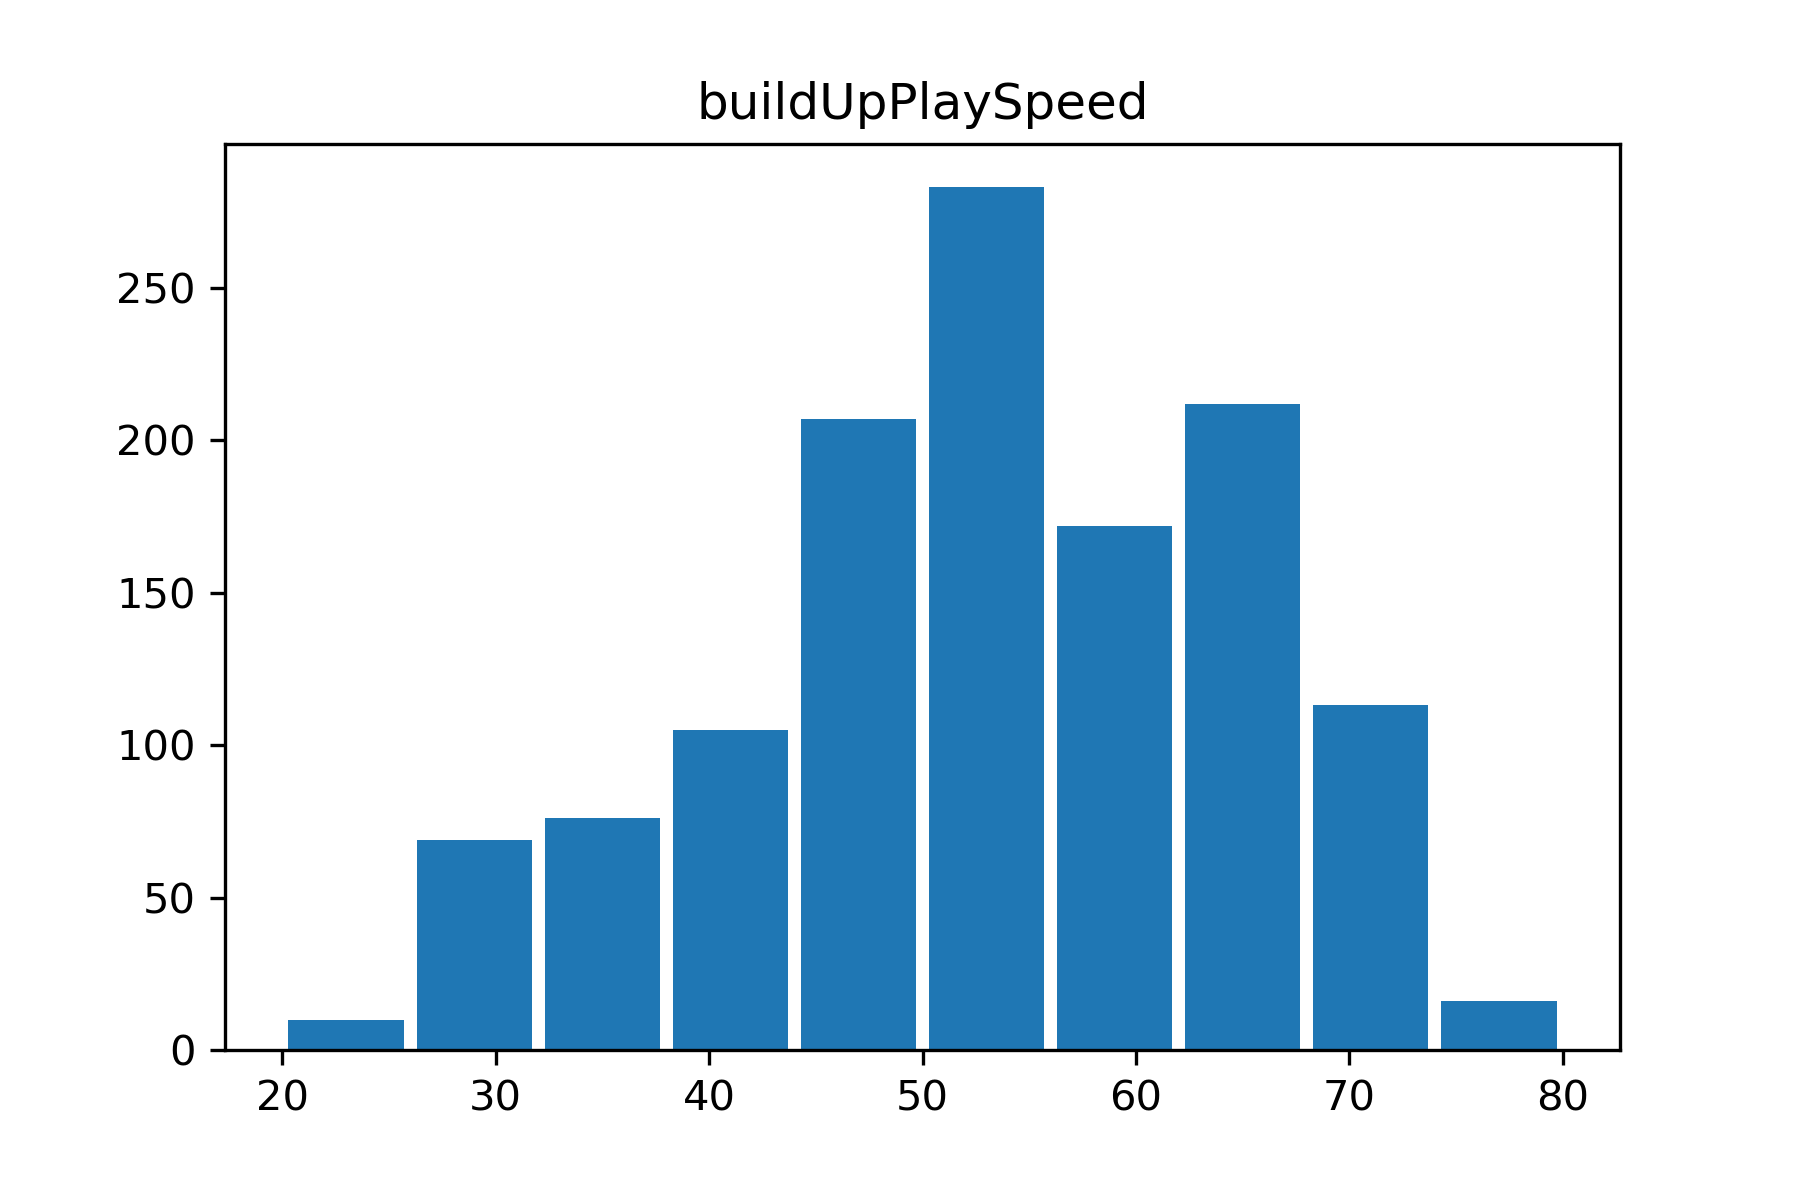
\includegraphics[width=40mm]{k-means_graphs/buildUpPlaySpeed.png} \\
(a) buildUpPlayDribbling & (b) buildUpPlayPassing & (c) buildUpPlaySpeed \\[6pt]
 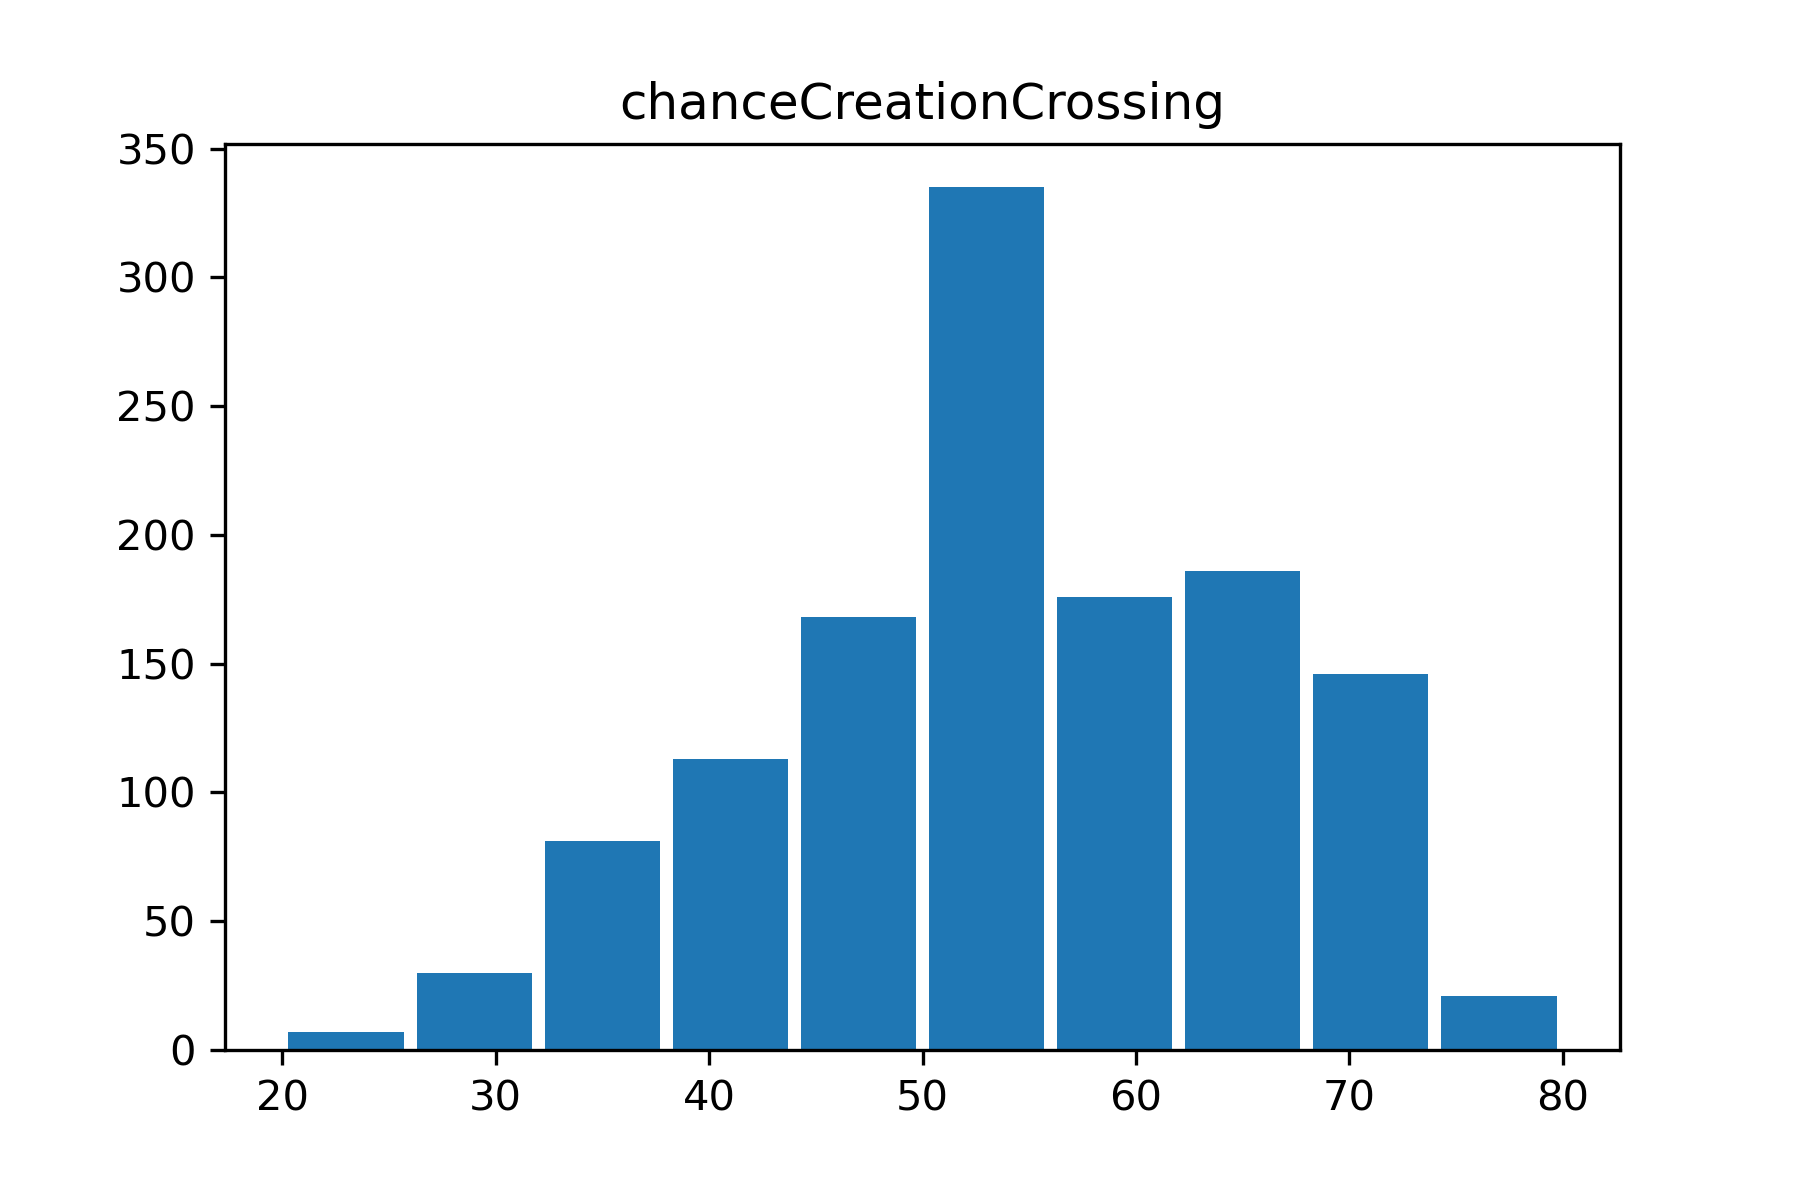
\includegraphics[width=40mm]{k-means_graphs/chanceCreationCrossing.png} &   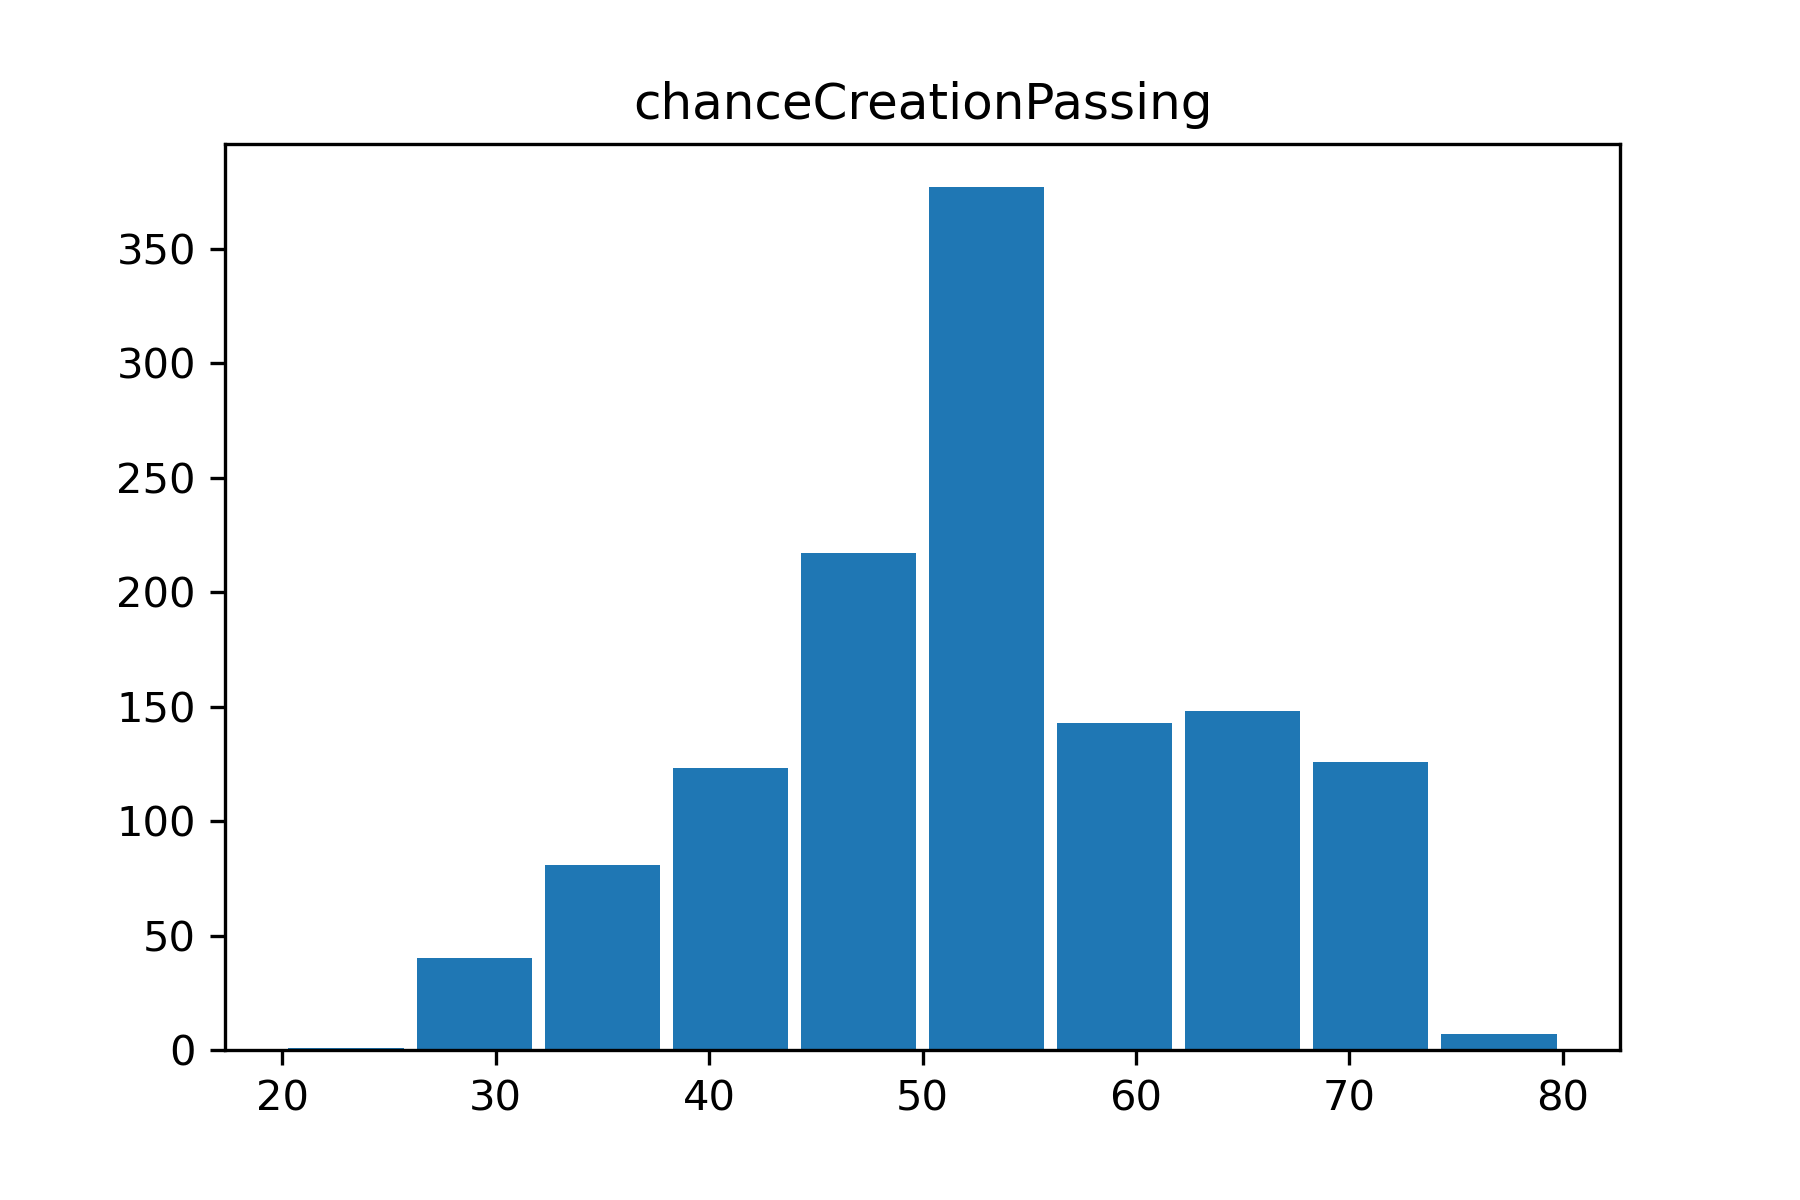
\includegraphics[width=40mm]{k-means_graphs/chanceCreationPassing.png} &   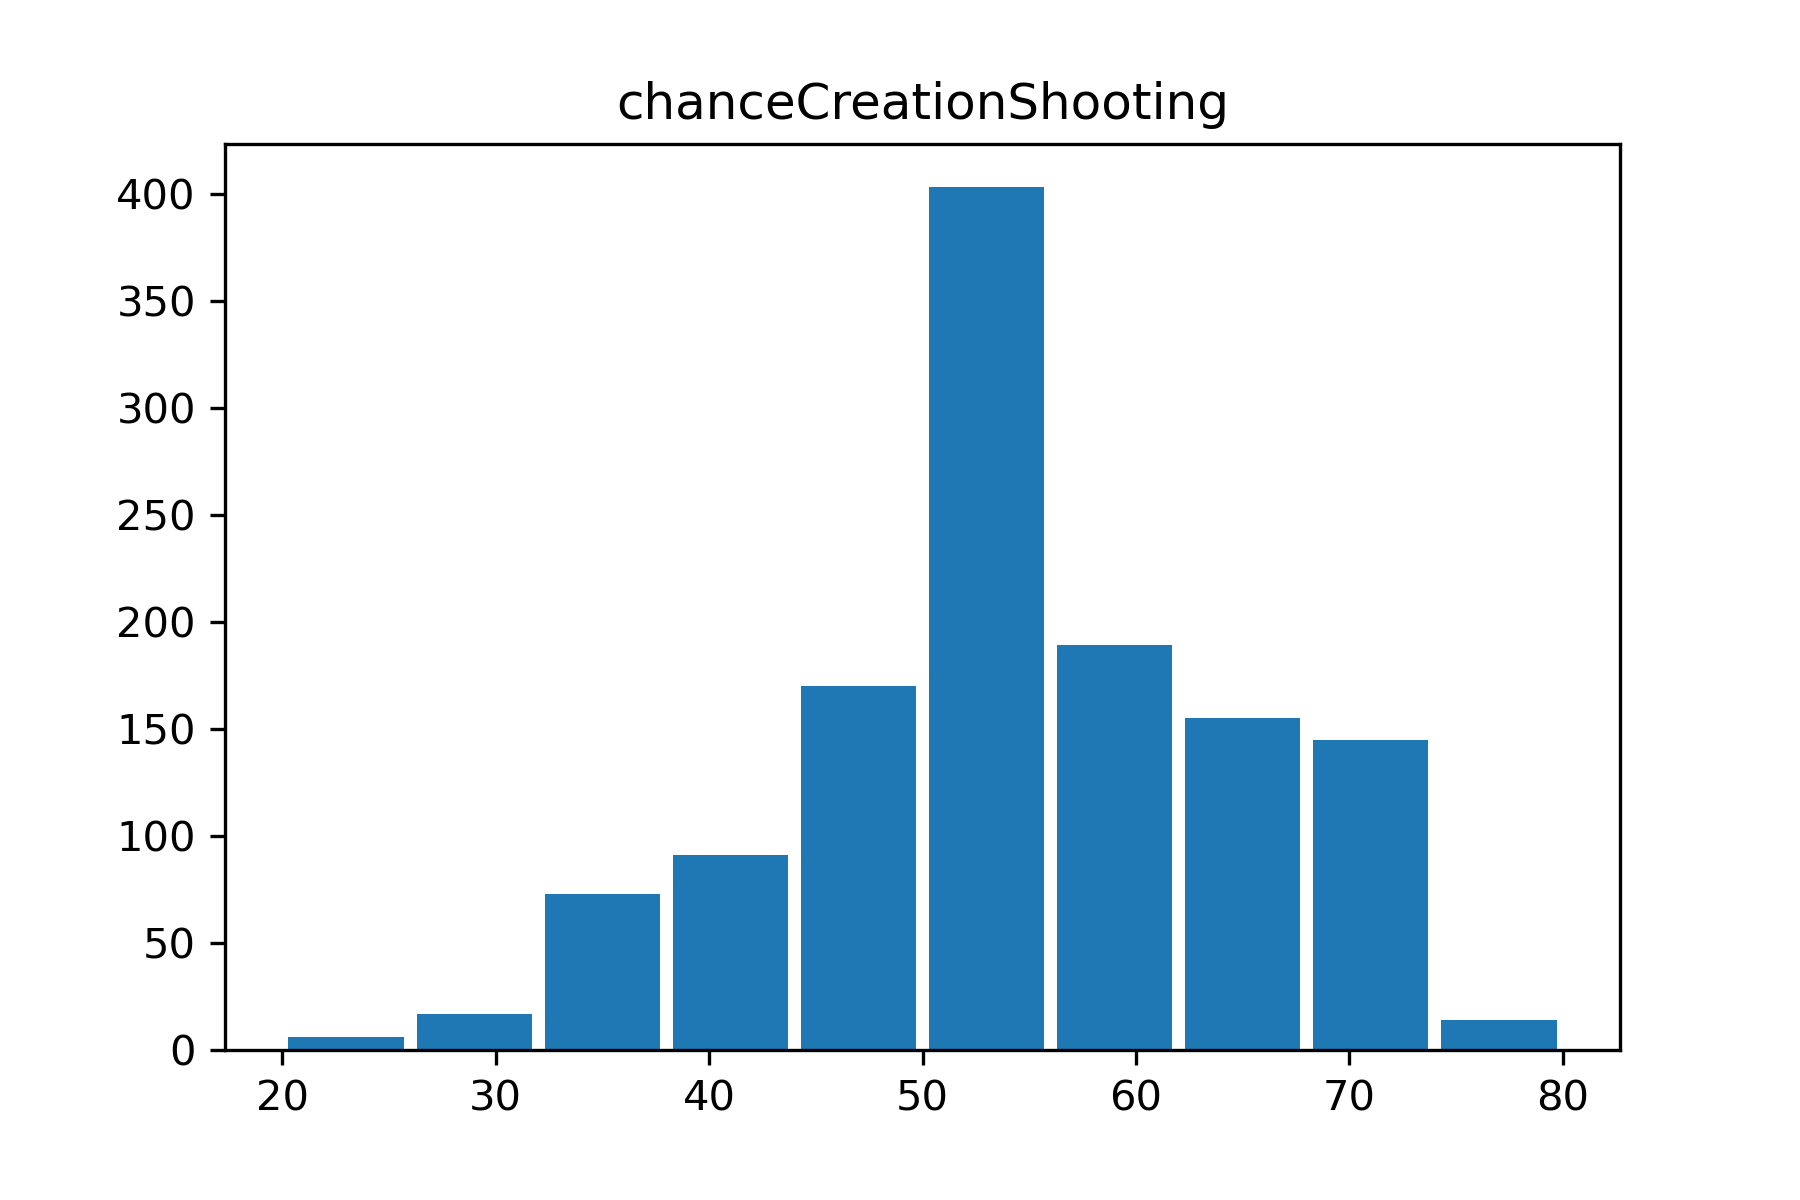
\includegraphics[width=40mm]{k-means_graphs/chanceCreationShooting.png} \\
(d) chanceCreationCrossing & (e) chanceCreationPassing & (f) chanceCreationShooting \\[6pt]
 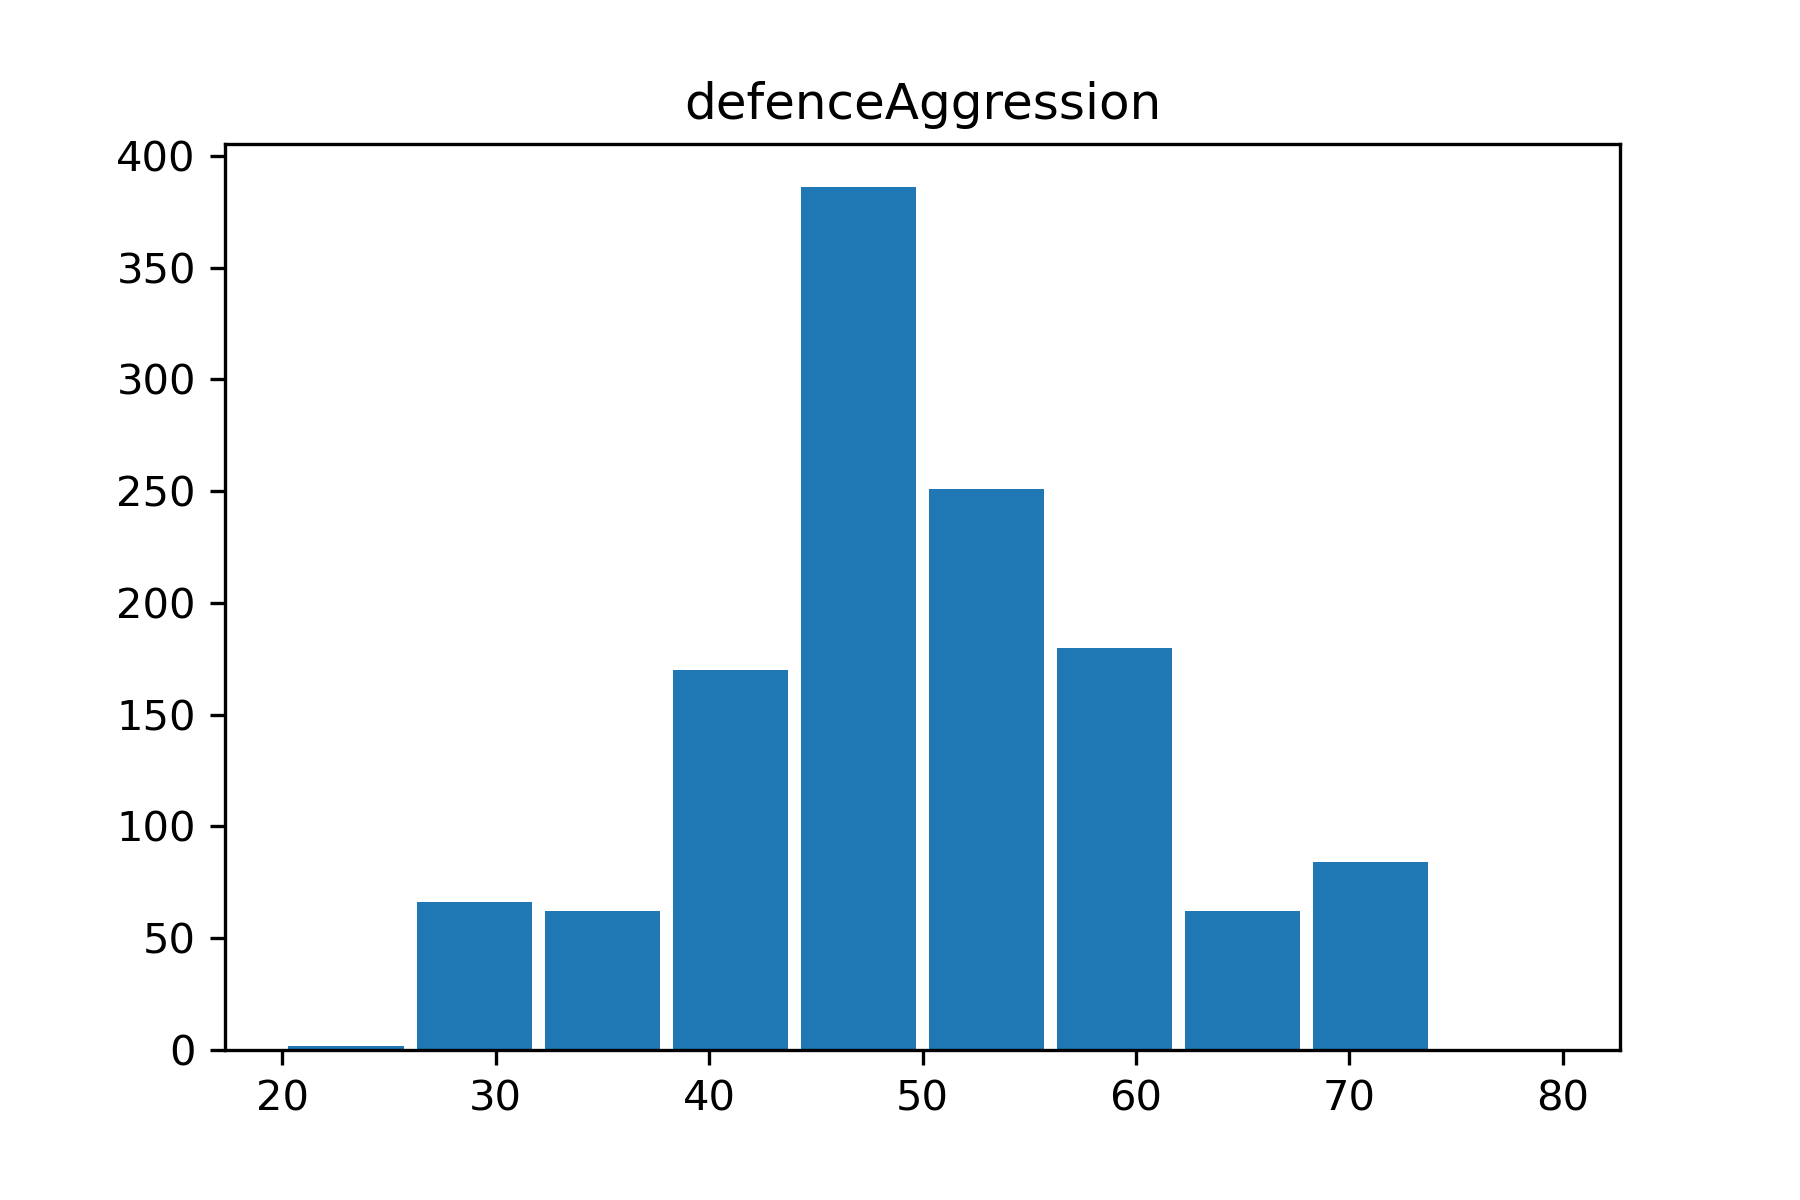
\includegraphics[width=40mm]{k-means_graphs/defenceAggression.png} &   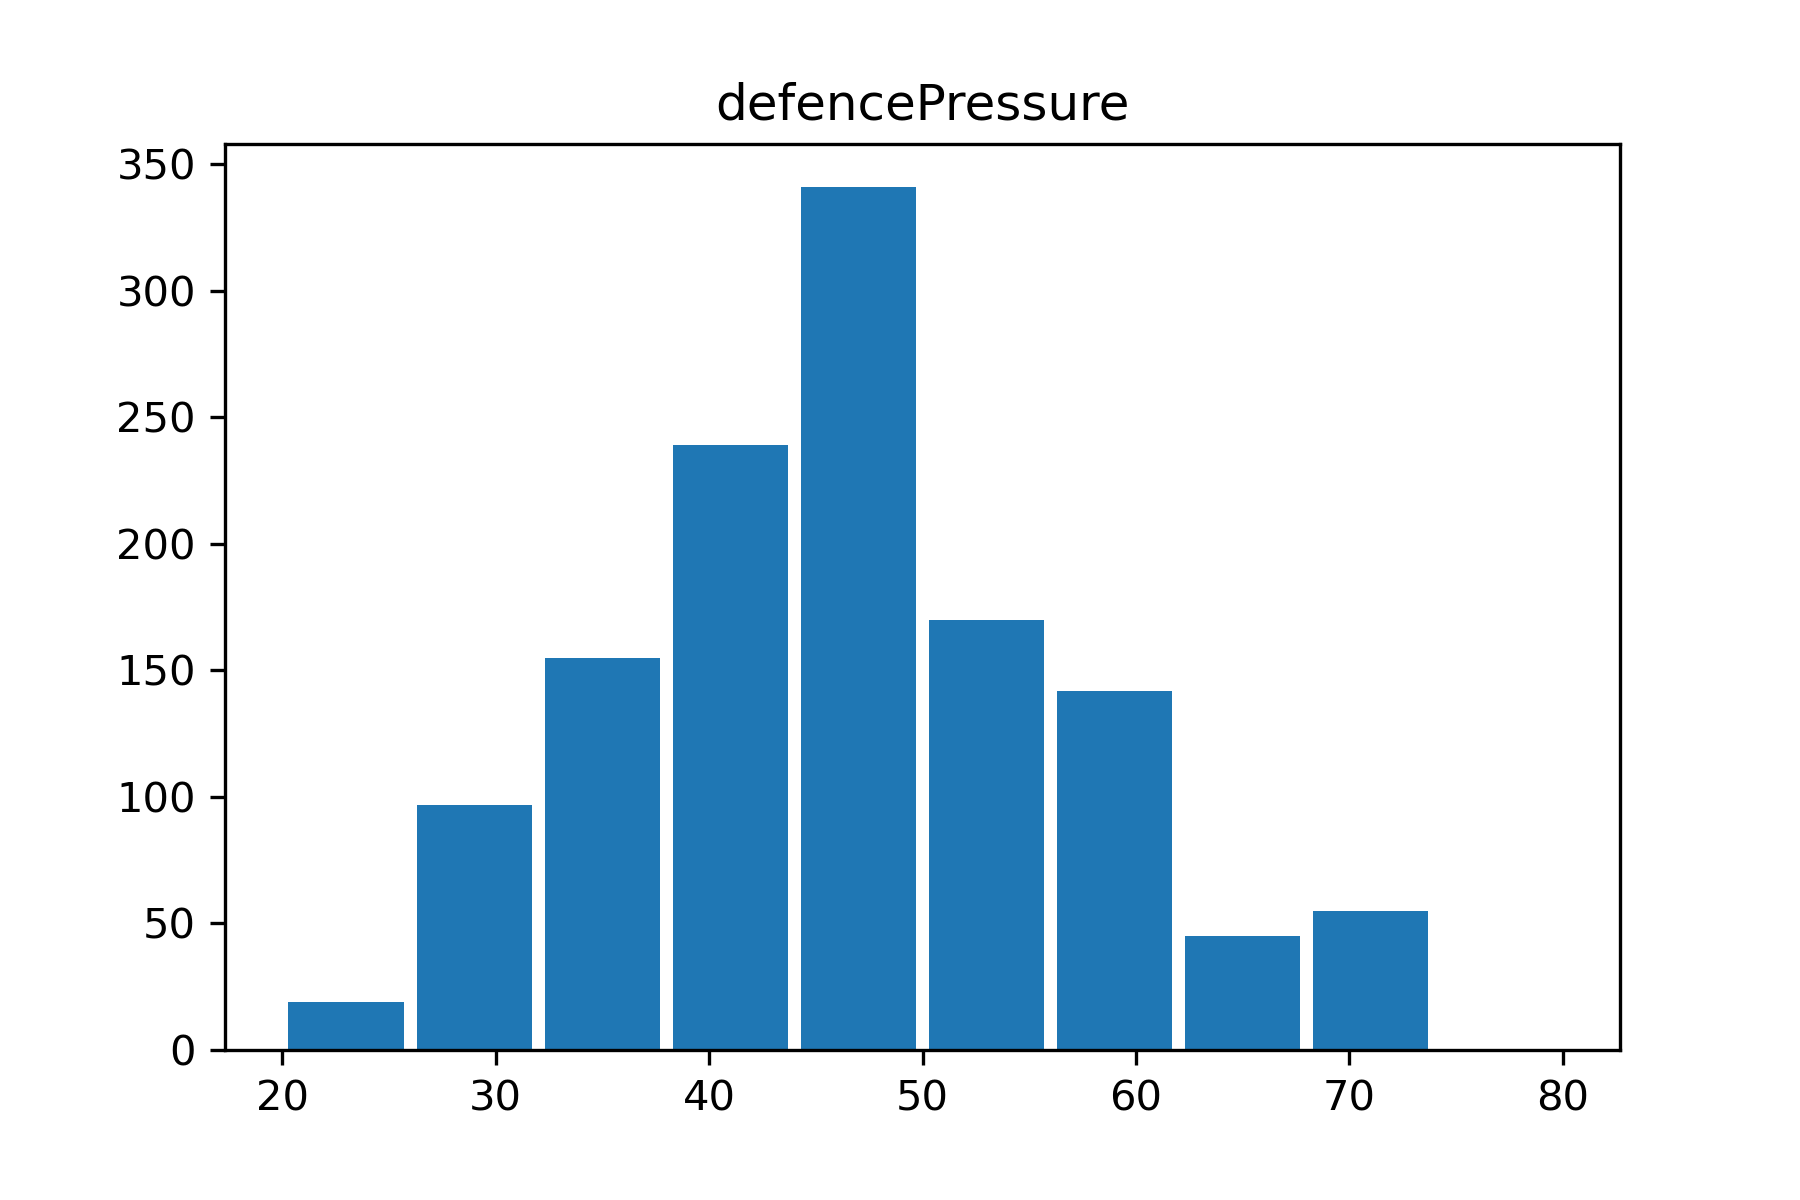
\includegraphics[width=40mm]{k-means_graphs/defencePressure.png} &   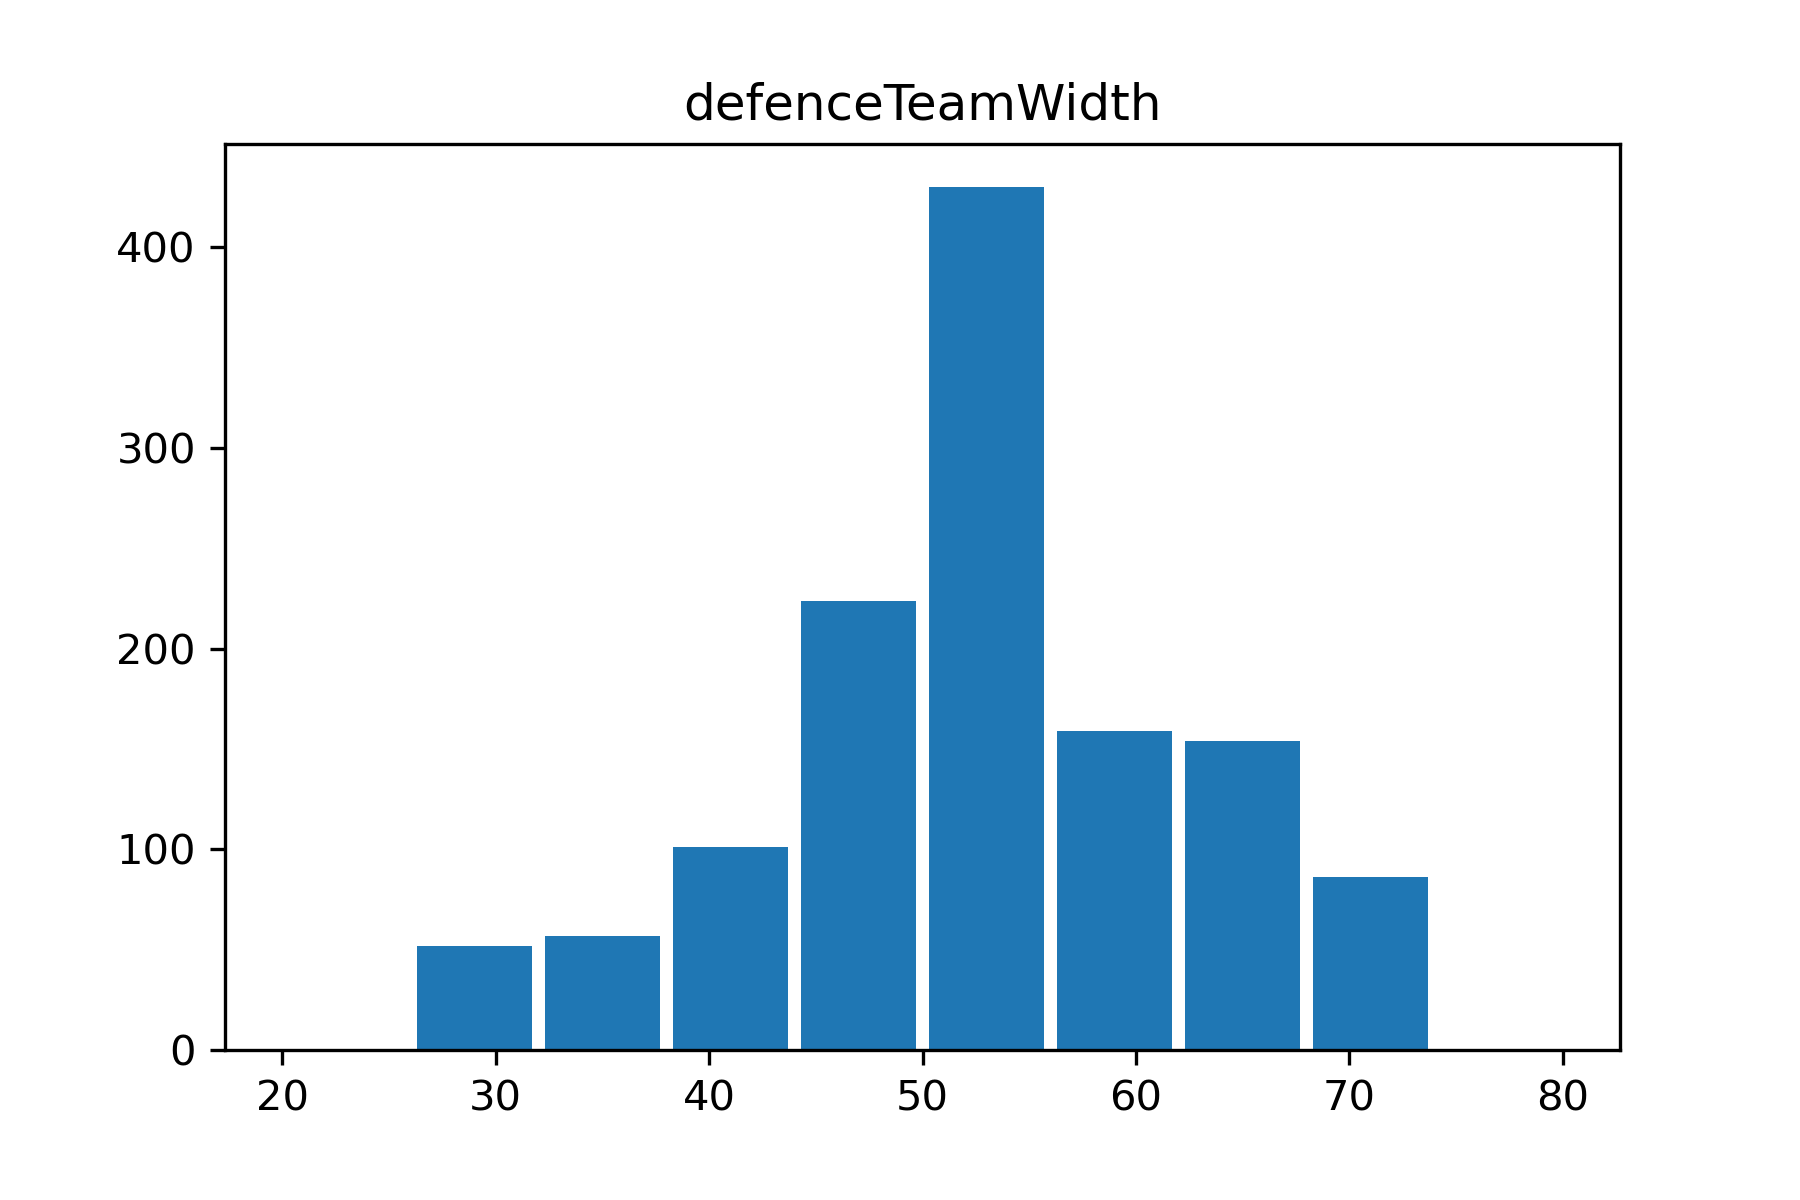
\includegraphics[width=40mm]{k-means_graphs/defenceTeamWidth.png} \\
(g) defenceAggression & (h) defencePressure & (i) defenceTeamWidth \\
\end{tabular}
\caption{Distribution of each feature used in the preliminary K-means analysis}
\label{fig:k-means}
\end{figure}

The number of clusters is a key variable in determining the usefulness and precision of the clustering algorithm. For our preliminary analysis, we use a simple "elbow curve" method to determine the appropriate number of clusters. The K-means algorithm is run on the data set with number of clusters varying from 1 to 50 and the overall fit score is examined, as shown in Figure \ref{fig:elbow}(a). We see that the precision of clustering increased rapidly as the number of clusters is raised from 1 to 10, and continued to increase at a lower rate with more than 10 clusters. Here, 10 clusters are the point where a balance between precision and categorizing power is reached.

\begin{figure}[H]
\centering
\begin{tabular}{cc}
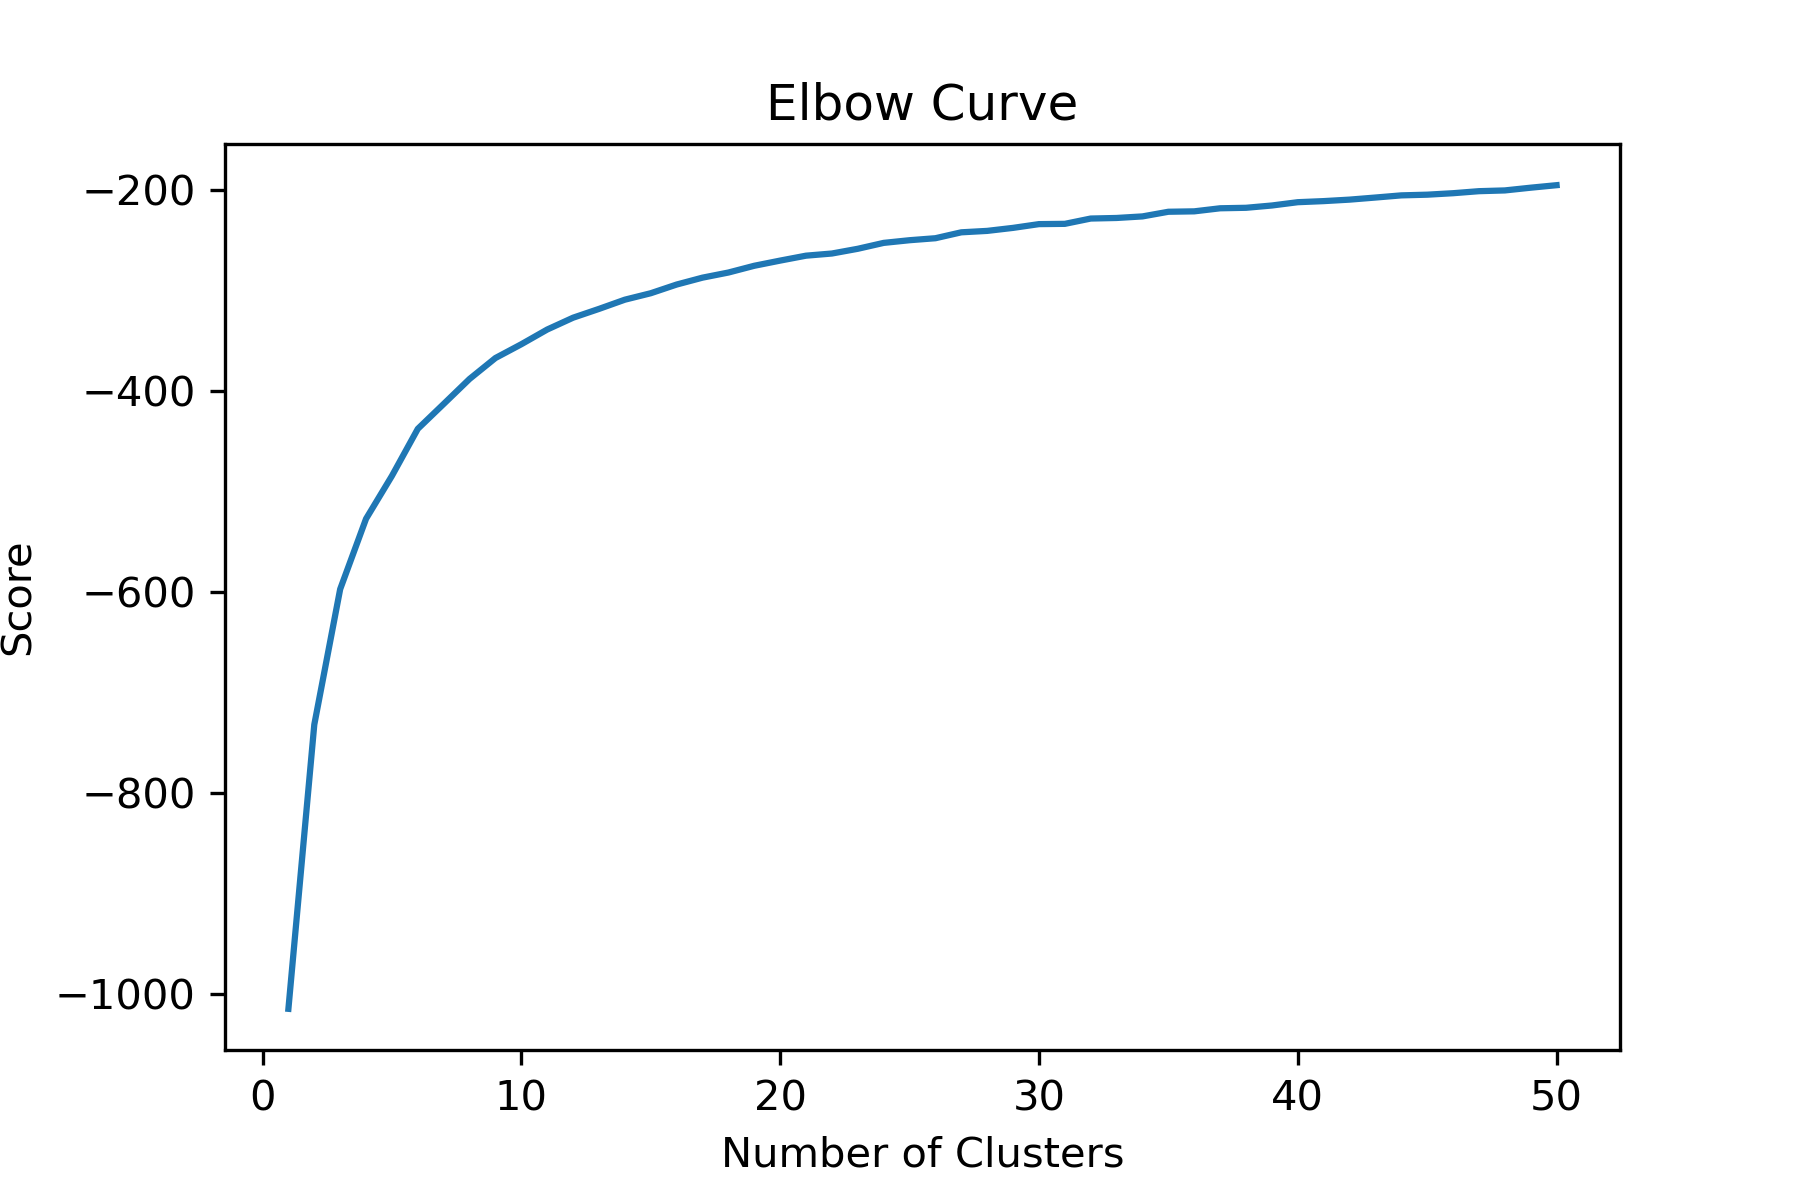
\includegraphics[width=70mm]{k-means_graphs/Elbow.png} &
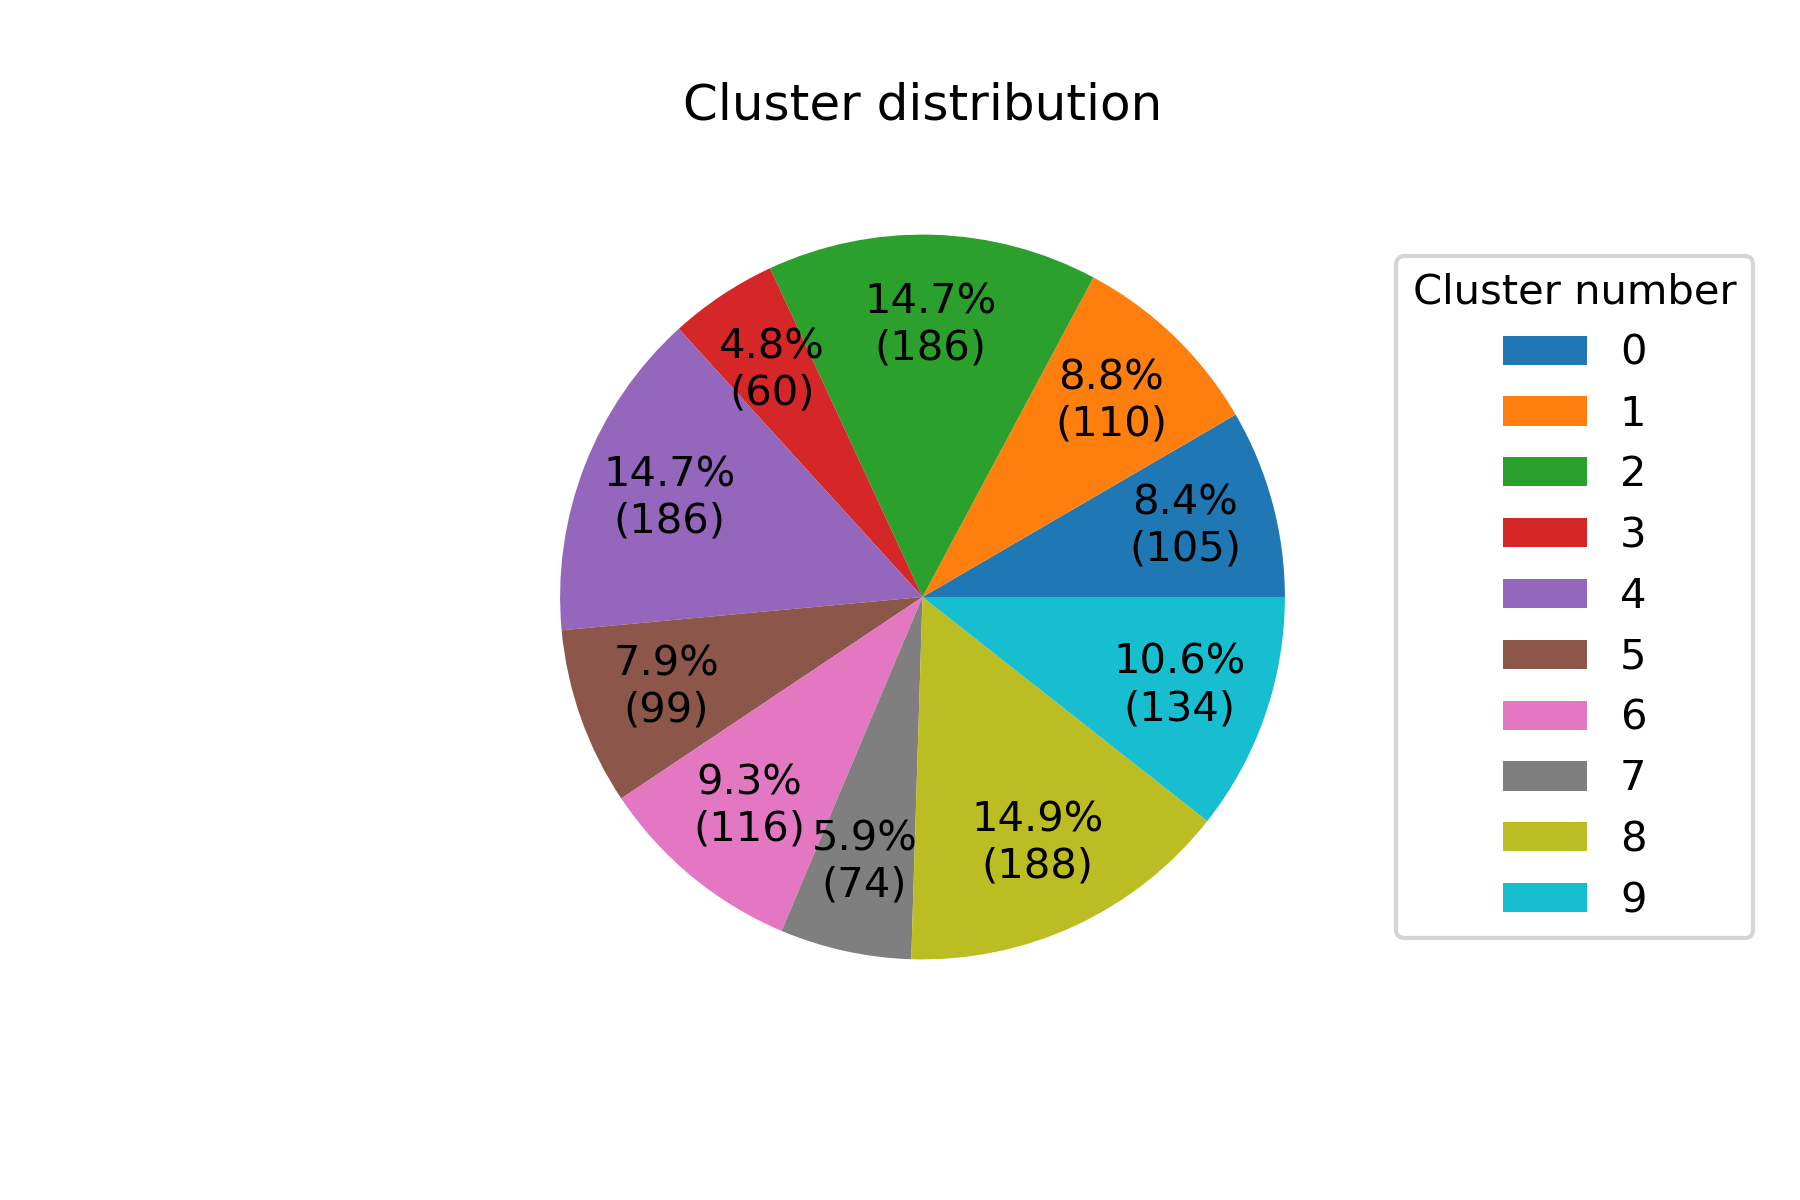
\includegraphics[width=90mm]{k-means_graphs/10clusters.png} \\
(a) Elbow curve & (b) Cluster sizes \\
\end{tabular}
\caption{Elbow curve and cluster sizes in the preliminary K-means analysis}
\label{fig:elbow}
\end{figure}

We note that the above clustering is performed on team attributes alone. Although no player attributes are taken into account, there is already a great diversity of team playstyles. The 10 clusters also have comparable sizes, which means the 10 metas we find here are all strategies that many teams can adapt to, as opposed to niche strategies that could only be played by one or two football players.

With this information, our assumption on teams having various metas is justified. That clutering gives poor precision (low score) when the number of clusters is lower than 10 is strong evidence that teams deploy different strategies and follow different playstyles. 

\subsection{Clustering Analysis}
The K-means algorithm is a special case of clustering with a mixture of Gaussians where all variances are equal and mixture weights are equal. This assumption is clearly suboptimal for many real-life applications where the distribution of clusters are not spherical. Hence, with our objective to find the best meta strategy by clustering team play styles, we improved our clustering methodology with Gaussian Mixture Model.

Using the identical min-max normalized dataset with all team and players attributes, we first performed hyper-parameter search for GMM. There are two parameters of interest: number of clusters and the type of covariance matrix. To evaluate the performance of GMM with different hyperparameters, we used penalized-likelihood criteria such as AIC and BIC. We chose both AIC and BIC together for model selection since a lower value of both AIC and BIC indicate a high data likelihood given the fitted GMM model and low overfitting.

By varying the number of clusters between 1 to 30 and the type of covariance matrix to be full, tied, and diagonal, we found that: 1) there is a large decrease in both AIC and BIC with 9 and 24 clusters 2) full covariance is computationally inefficient, and diagonal covariance type is best suited for meta strategy clustering (Fig \ref{fig:gmm}).

\begin{figure}[H]
\centering
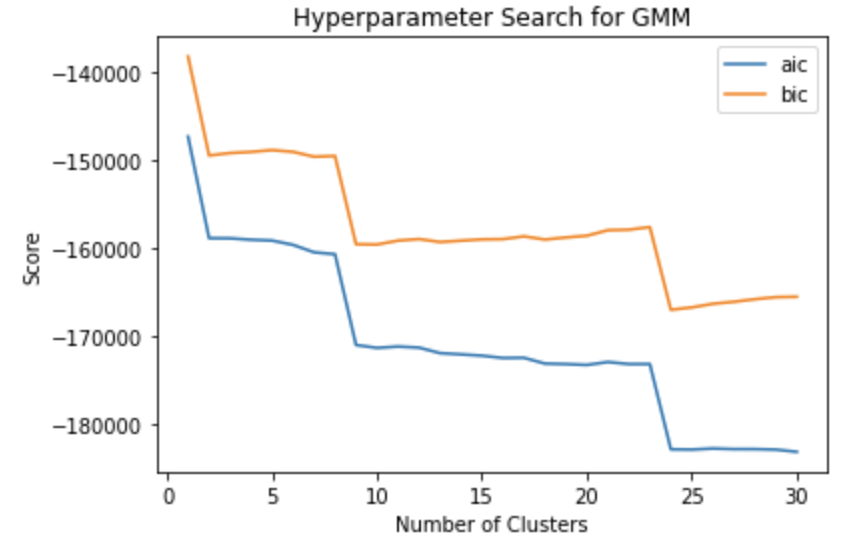
\includegraphics[width=.5\textwidth]{gmm.png}
\caption{Finding the optimal number of clusters (9, 24) with diagonal covariance matrix in GMM, measured by AIC and BIC.}
\label{fig:gmm}
\end{figure}

Hence, we formed 9 and 24 meta strategies and counted the number of team play styles in each meta strategy. We can see that 9 clusters provide a more general summary of meta strategy but 24 clusters provide a more detailed and balanced description of different meta strategies (Fig \ref{fig:gmm_count}). We therefore decide to analyze meta interactions with clustering results of \textbf{both} 9 and 24 meta strategies.

\begin{figure}[H]
\centering
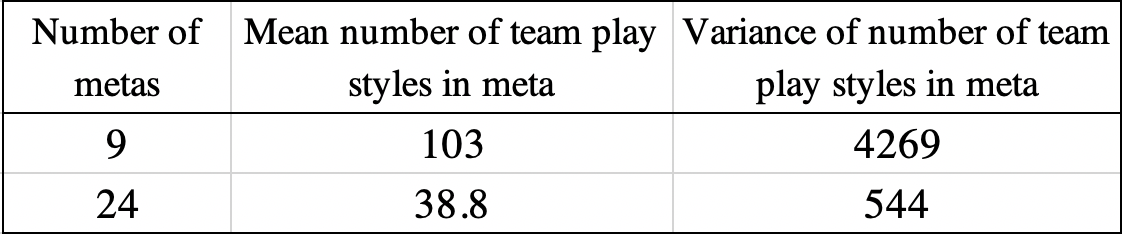
\includegraphics[width=.7\textwidth]{gmm_count.png}
\caption{Summary statistics for number of team play styles within each meta strategy after GMM clustering.}
\label{fig:gmm_count}
\end{figure}

\subsection{Inter-Meta Analysis}
With the meta strategies from GMM, we want to understand and interpret the different meta strategies and how they interact with each other in football matches. We assigned each of the two teams at a match event to a meta strategy by looking for the closest clusters for the team's play style. Since we treated different entries of the same team's attributes as separate team instances, the same team (identified by team id) could still be assigned to different metas due to changes in playstyle or player attributes at different matches. This treatment allows for maximum accuracy in categorizing the playstyle of a team in a given point in time.

To analyze the winning relations between all metas, we take a pair $(u,v)$ of meta strategies and calculate the expected number of goals scored by all teams in $u$ against all teams in $v$. If the expected number of goals for pair $(u,v)$ is positive, that means teams playing with meta strategy $u$ on average scores more than teams playing with meta strategy $v$. By calculating the expected number of goals between all pairs of meta, we can generate a weighted directional graph $G$ between all meta strategies, where a vertex $v\in[0,numCluster-1]$ is a meta strategy, and an edge $e:u\rightarrow v$ with weight $w_e$ means teams with meta $u$ has a positive expected number of goals $w_u$ against teams with meta $v$.

We first applied our inter-meta winning relation graph on the 9 meta strategies we found with GMM (Fig \ref{fig:gmm9}). From the weighted directional graph, we can see clear and diverse interactions among meta strategies, such as meta strategy 7 has a high number of goals against 5, but is countered by meta strategy 3. We highlighted edges with large weights, meaning a large difference in the expected number of goals between the two strategies at the ends of the edge.

\begin{figure}[H]
\centering
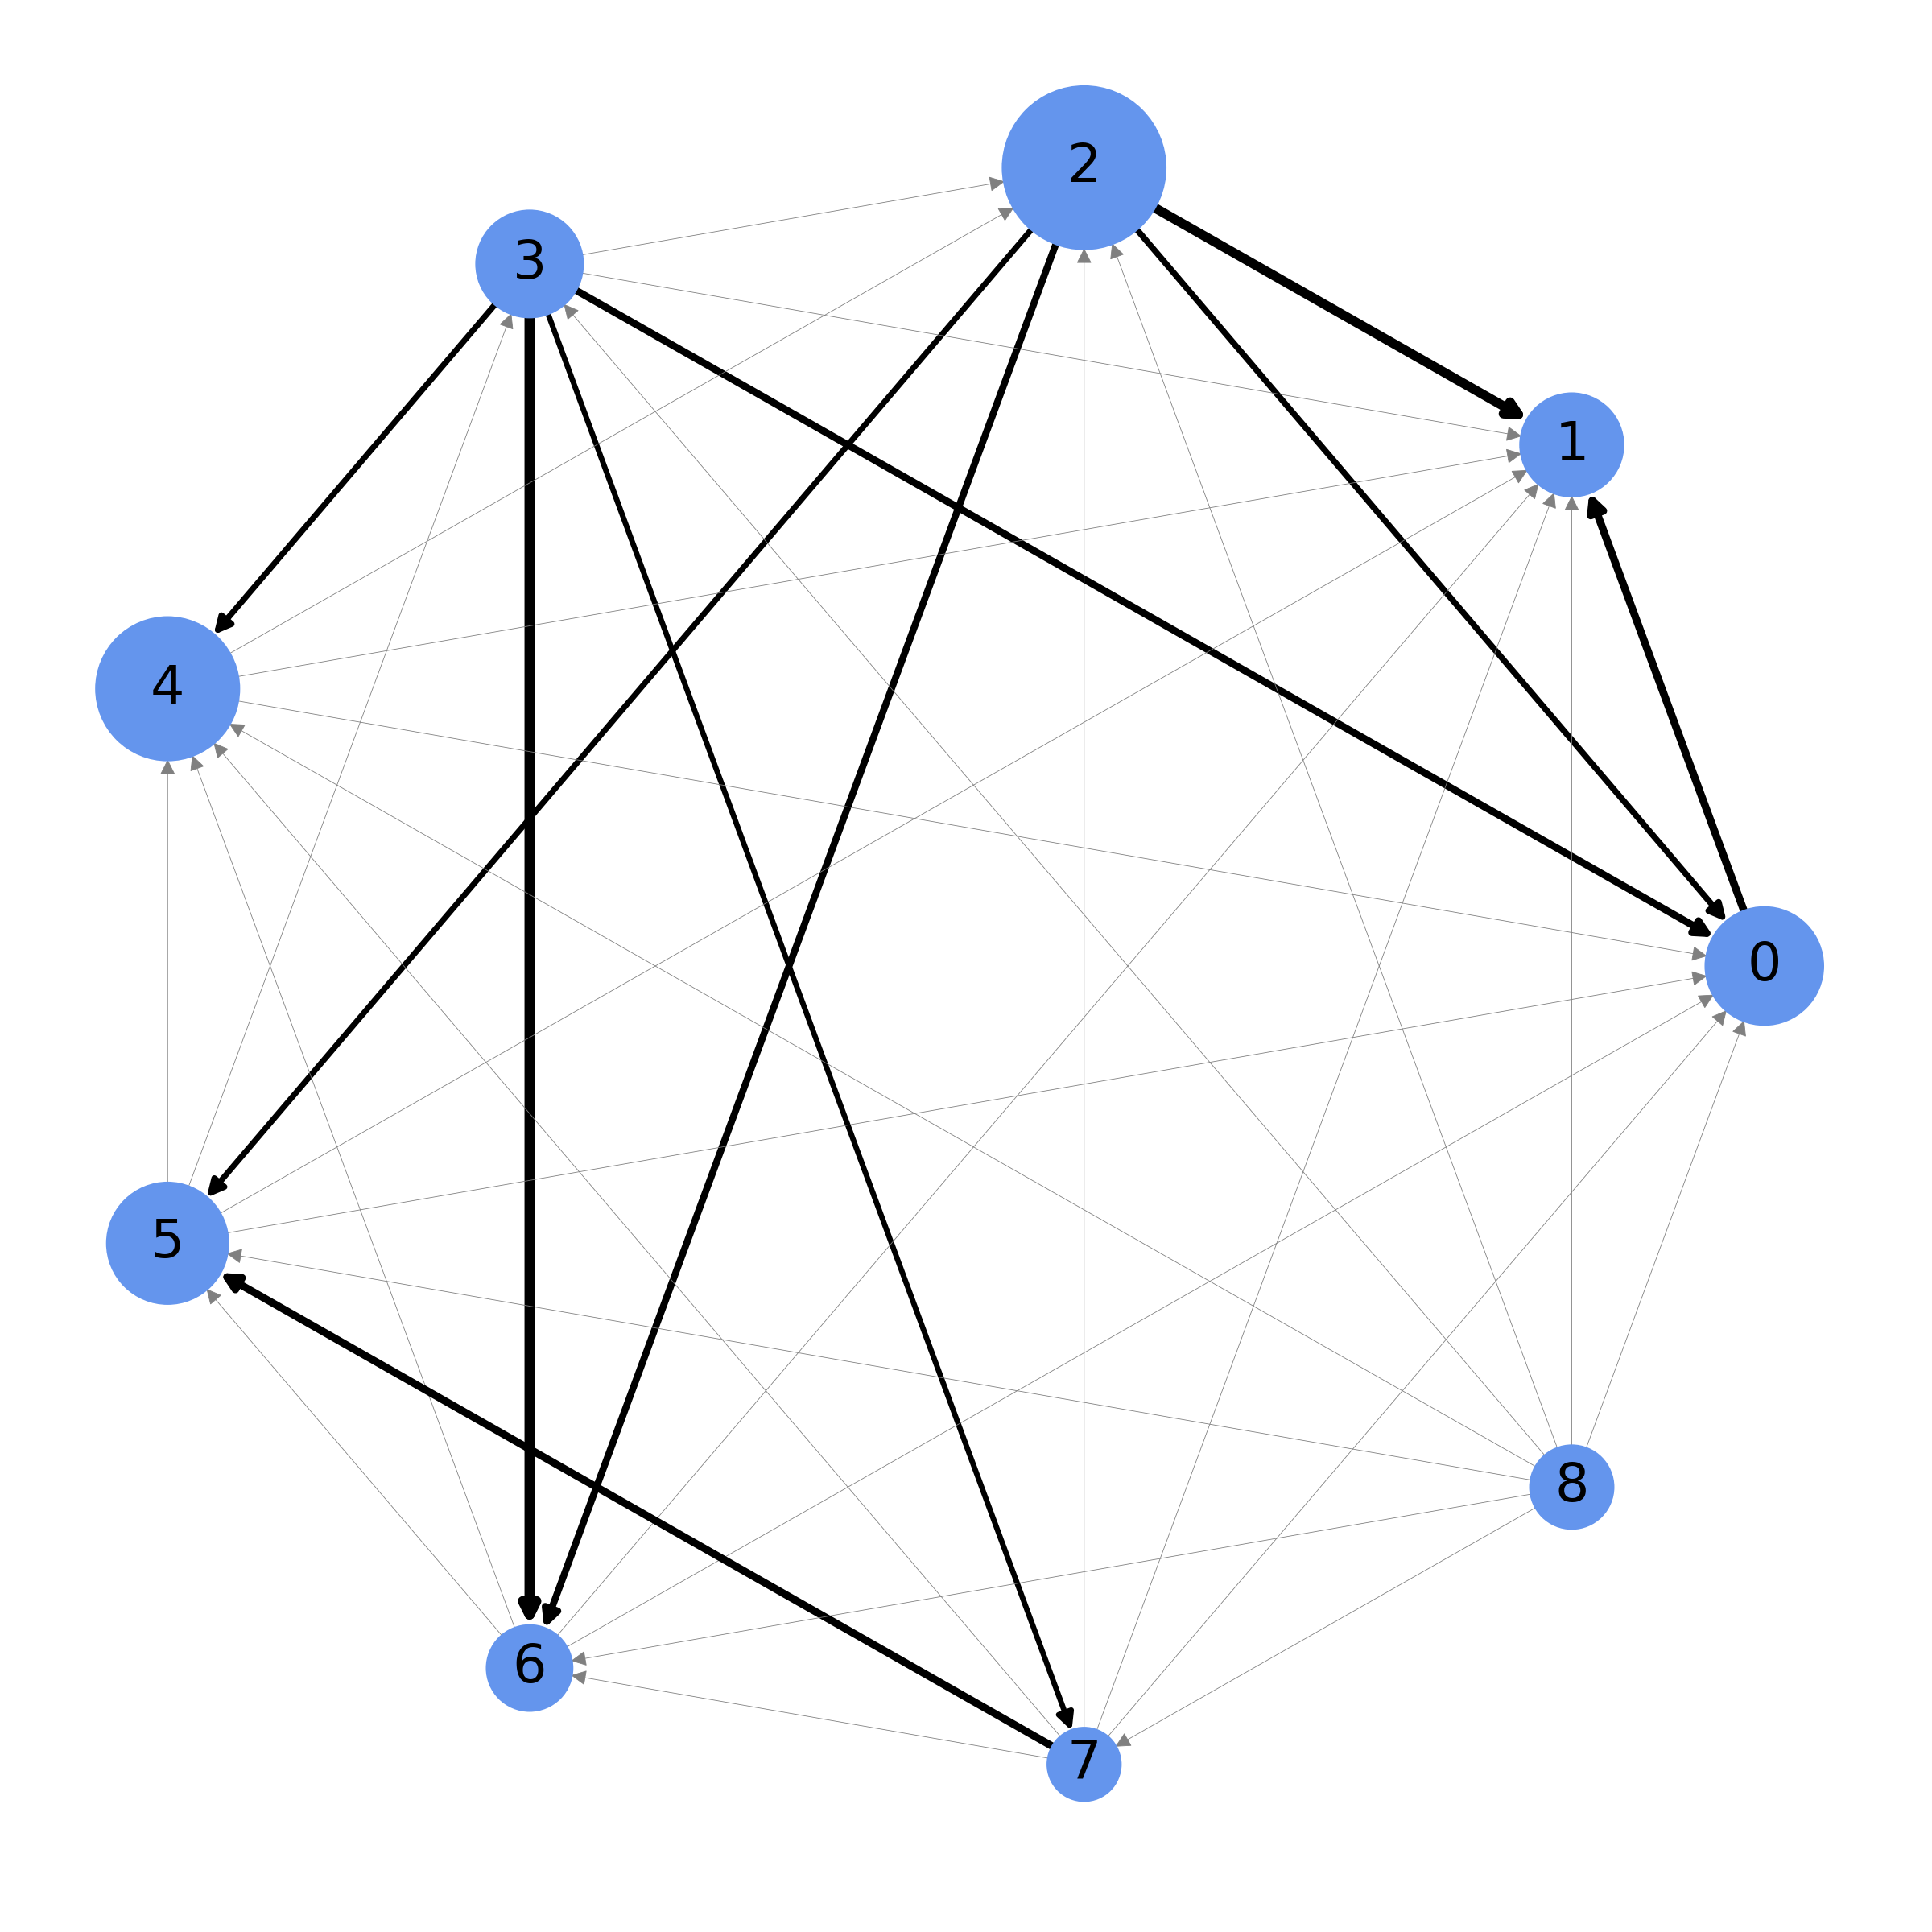
\includegraphics[width=.5\textwidth]{gmm9.png}
\caption{Inter-meta winning relations between 9 GMM clusters.}
\label{fig:gmm9}
\end{figure}

We are then interested to see interactions between the more clearly defined and distinct 24 meta strategies found by GMM. Using the same algorithm, we generated the inter-meta winning relations between 24 meta in Fig \ref{fig:gmm24}:

\begin{figure}[H]
\centering
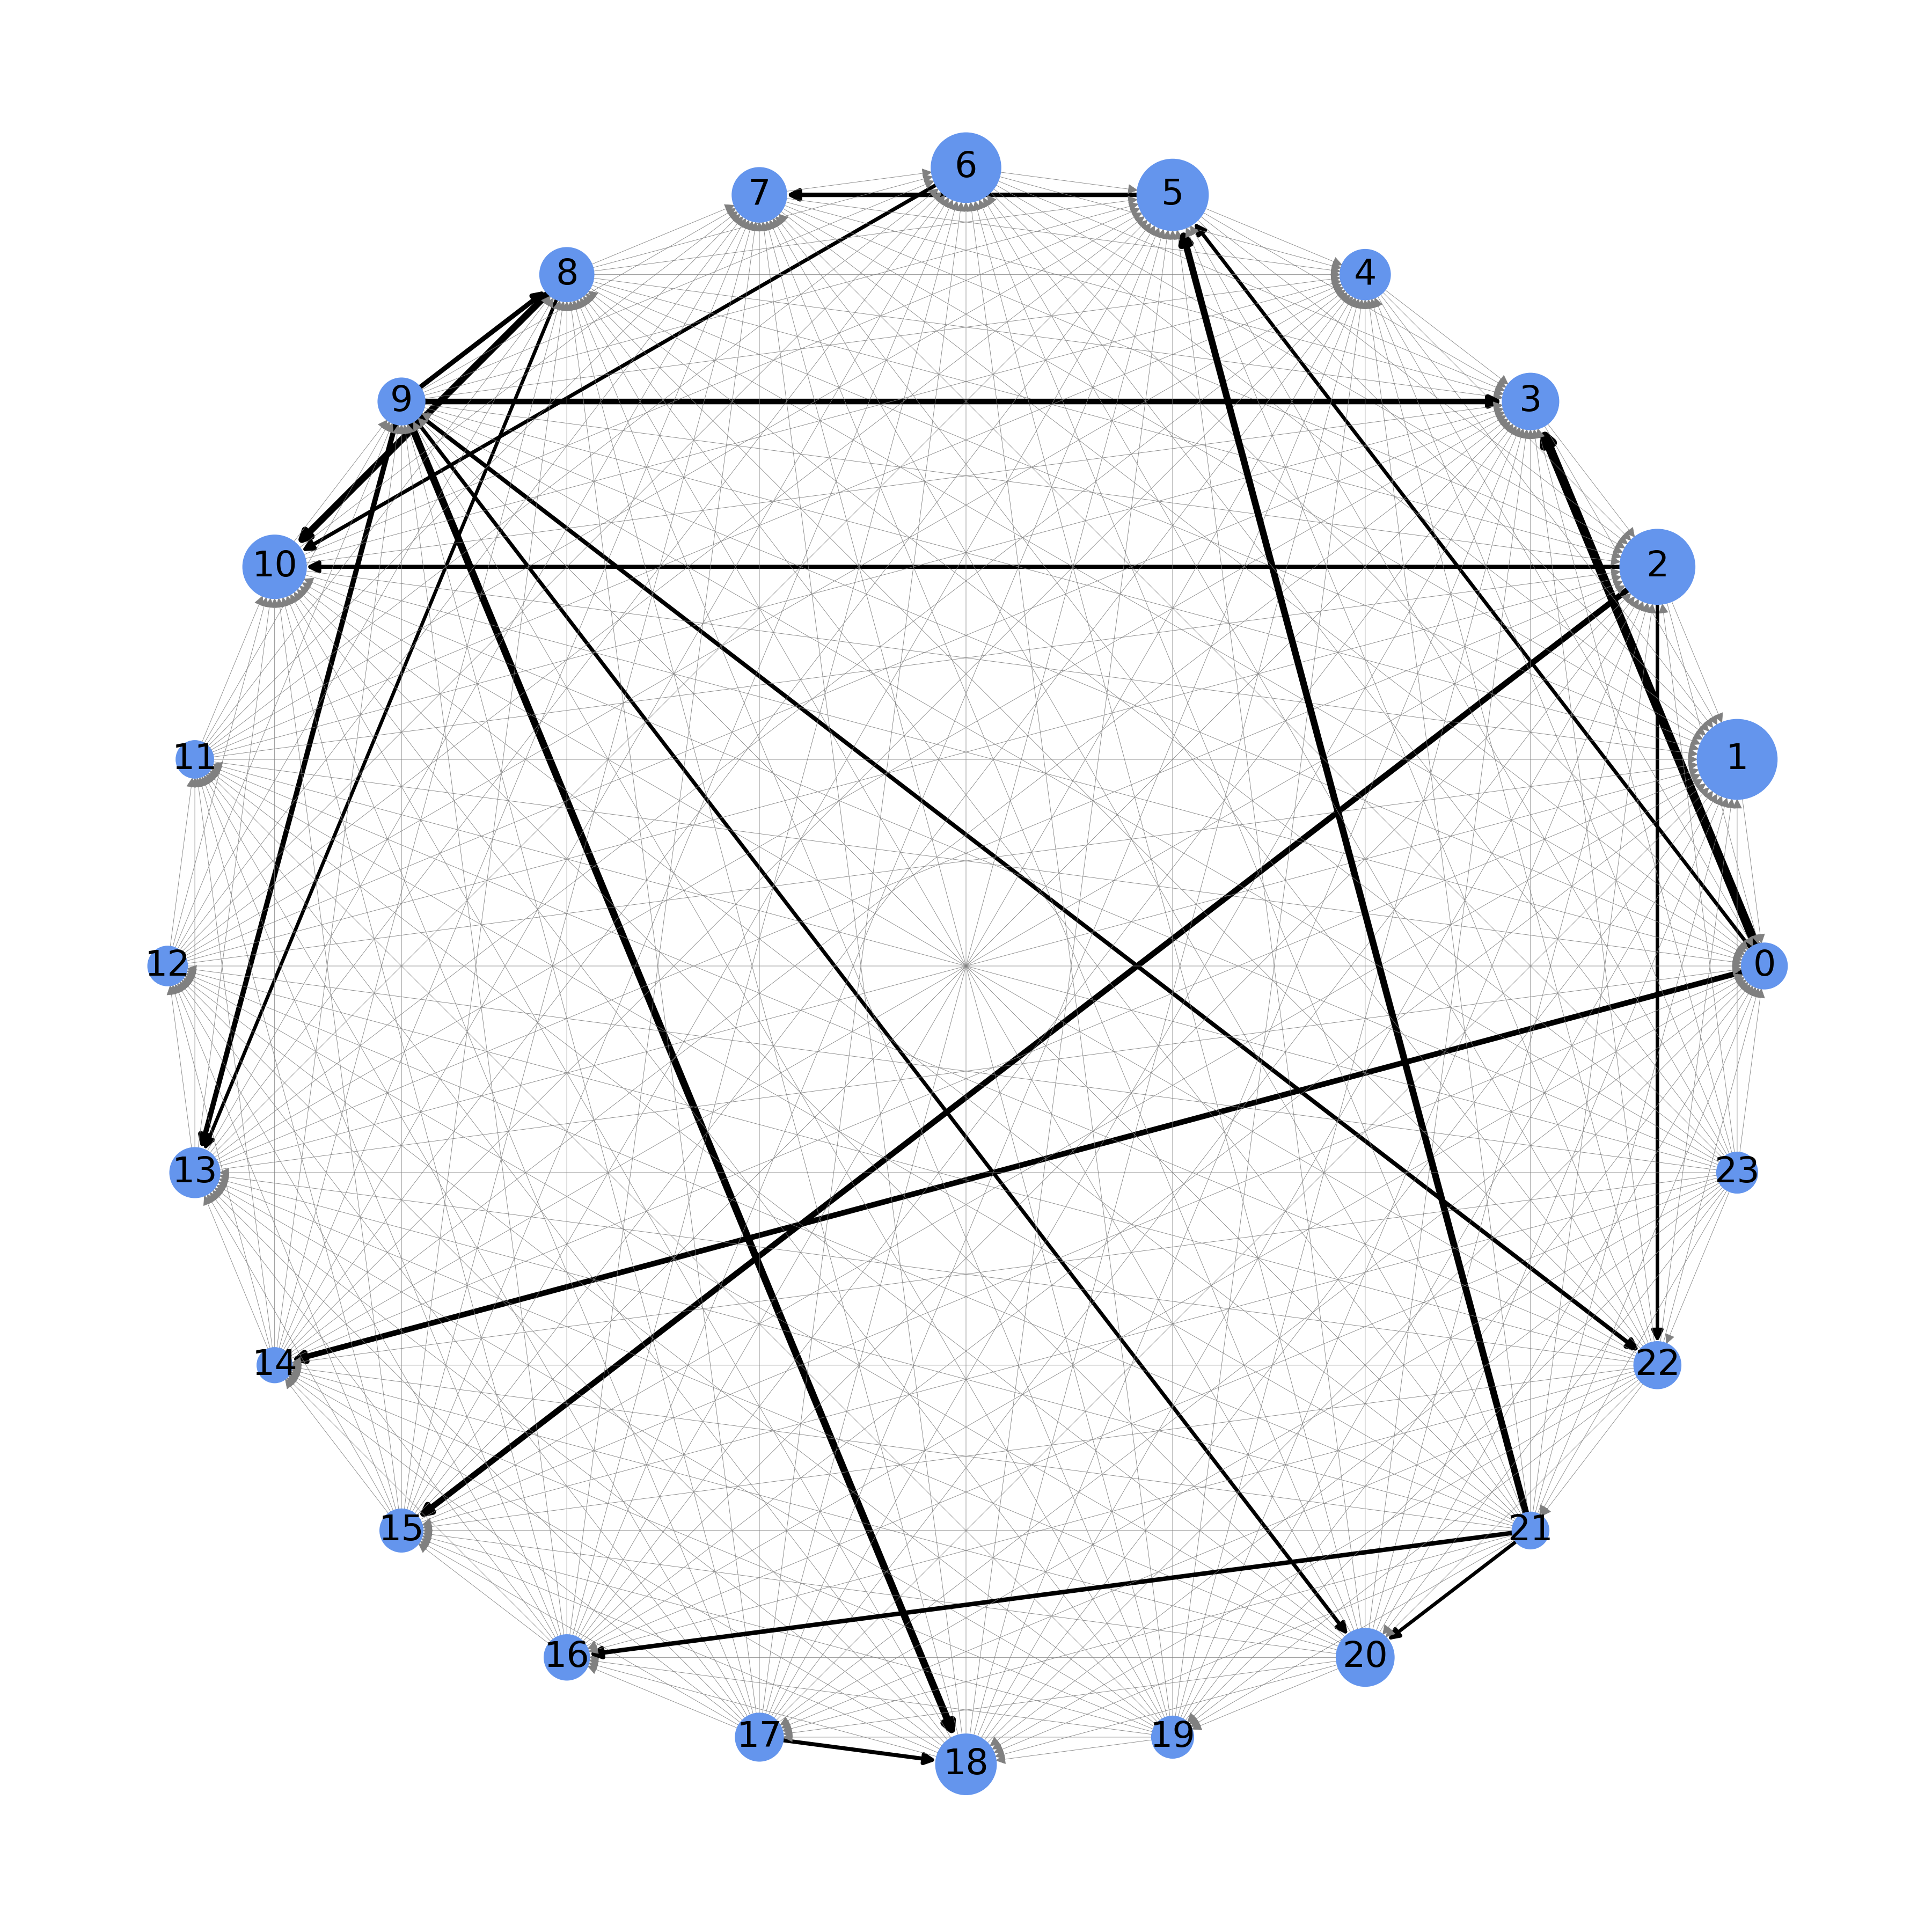
\includegraphics[width=.7\textwidth]{gmm24.png}
\caption{Inter-meta winning relations between 24 GMM clusters.}
\label{fig:gmm24}
\end{figure}

Despite the complex interaction between many pairs of the 24 meta strategies, we observe edges with significantly higher weights, indicating an even clearer patterns of inter-meta interactions and a large impact of meta strategy choice on the expected number of goals in a game. We also see some superior meta strategies, such as meta 9, that delivers a large number of goals against many other metas such as 10, 3, and 8.  Fig \ref{fig:gmm24} is also helpful as it points out interesting meta strategies with large impact on game outcomes for us to analyze later. Hence, we will proceed with only using the meta strategies from GMM with 24 clusters.



\subsection{Validation and Recommendation Testing}
By analyzing inter-meta interaction, we gained a deeper understanding of how play styles that fall under one meta strategy are effective against play styles in some but not other meta strategies.

To verify results from inter-meta interaction and its value in real-life match strategizing, we seek to answer the following question: \textbf{given an opponent's meta strategy, does using the best counter meta from our meta interaction graph gives a statistically significant higher expected number of goals, than using a random meta strategy?} Here we define the best counter meta as the meta with the highest expected number of goals against the opponent's meta strategy in our meta interaction graph.

First, playing against a given meta strategy, we calculated the expected number of goals scored by an average counter meta strategy and the expected number of goals scored by the best counter meta strategy (Fig \ref{fig:countermeta}). For example, if our opponent is playing meta 1, a team using a random meta is expected to score 0.23 goals against our opponent. However, using the best counter meta suggested by our meta interaction graph, we should adopt meta strategy 9 and will have an expected number of goal of 1.36 against our opponent.

\begin{figure}[H]
\centering
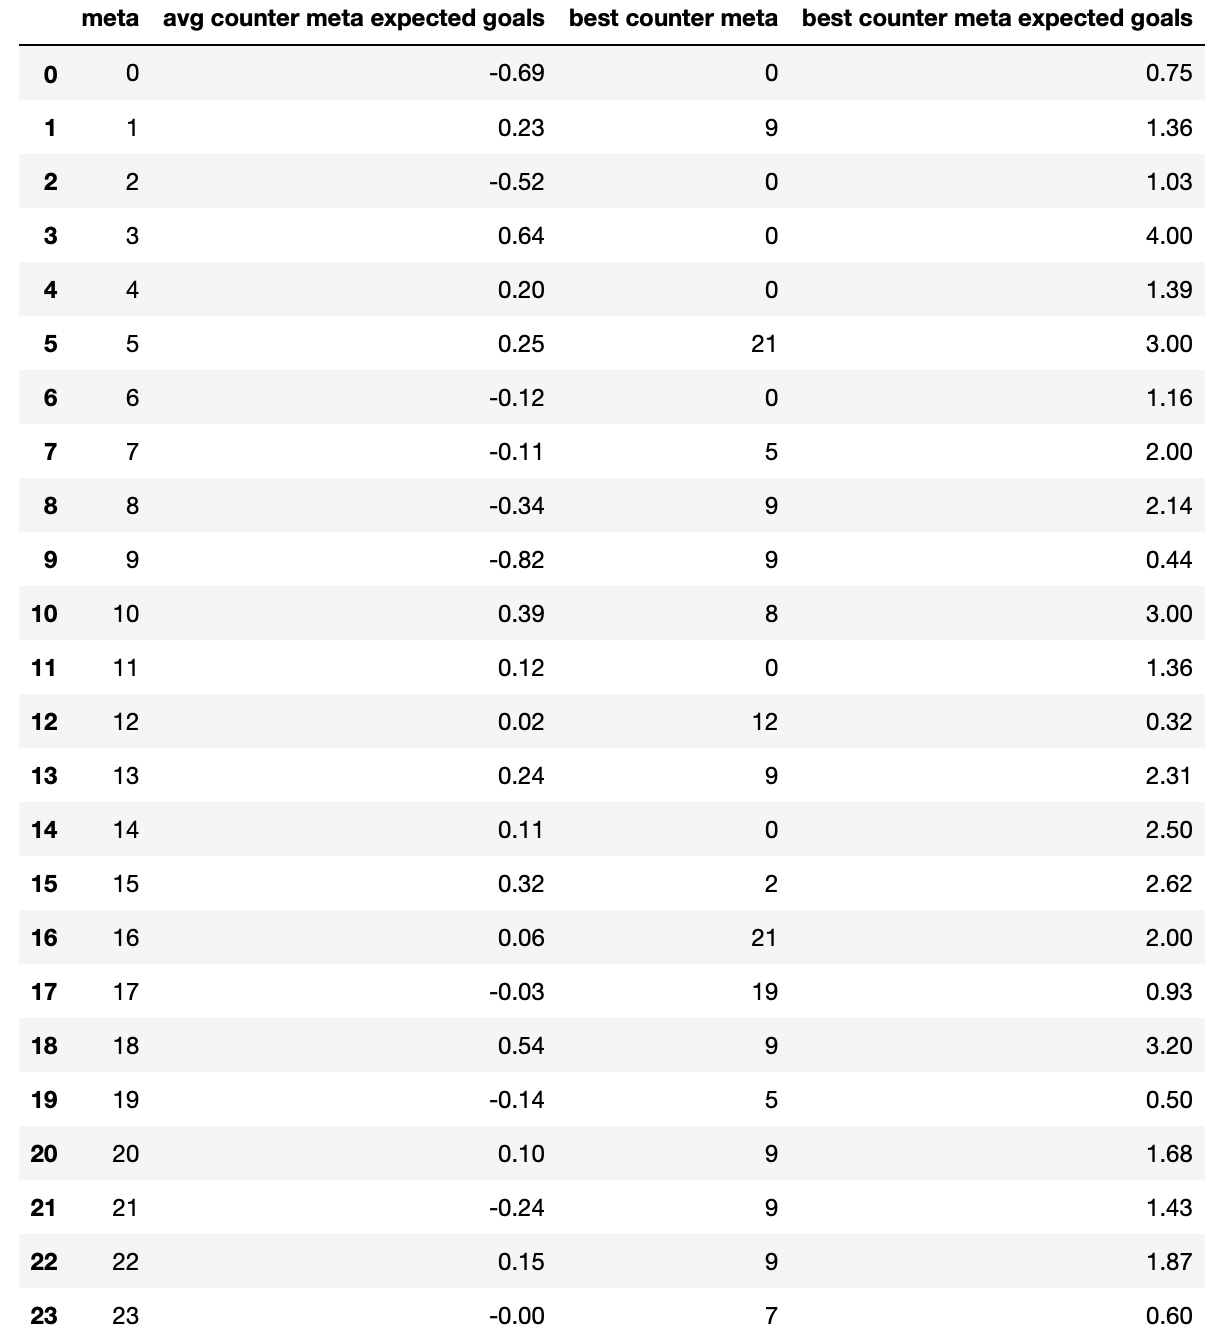
\includegraphics[width=.7\textwidth]{countermeta.png}
\caption{The expected number of goals by the best counter meta is significantly higher than that by an average counter meta against a given meta strategy}
\label{fig:countermeta}
\end{figure}

To answer the question above, we perform a hypothesis testing by comparing the expected number of goals scored by an average counter meta and best counter meta. Although we have two samples (one for the average counter meta and one for our best counter meta), all observations are dependent to each other. Hence, we conduct a matched pair comparison by testing on the difference between the two samples. Assuming the number of goals is independent across different clusters and given a specific opponent meta, we wish to test

\begin{center}
\(H_{0}\): The best counter meta recommended by our analysis\\
does not increase the expected number of goals.
\end{center}

versus

\begin{center}
\(H_{1}\): The best counter meta recommended by our analysis\\
does increase the expected number of goals.
\end{center}

Mathematically, we test

\begin{center}
\(H_{0}: E_{g}^{BCM} - E_{g}^{AVG} = 0\) versus \(H_{1}: E_{g}^{BCM} - E_{g}^{AVG} > 0\)
\end{center}

Since the sample size is small (n=24<30) and the population variance is unknown, we use t-statistic for hypothesis testing. Under the null hypothesis,

\[T=\overline{(E_{g}^{BCM} - E_{g}^{AVG})} \frac{\sqrt{n}}{S}~t_{n-1}\]

And we reject the null hypothesis if

\[T>t_{n-1, \alpha/2}\]

where \(S\) is sample variance, \(t_{n-1}\) is the Student's t-distribution with degree of freedom \(n-1\), and \(\alpha=0.05\). Plugging in the values in Fig \ref{fig:countermeta}, we indeed verify that the null hypothesis is rejected at the 0.05 significance level. There is statistically significant evidence that our analysis is capable of giving recommendations that increase the expected number of goals against a known opponent meta.

This result is highly non-trivial. Our model of selecting the best counter meta is immediately relevant to a team's manager: If they knew the meta strategy their opponent's team is playing, they could see if the best counter strategy is possible for their team. In cases where a certain strategy might not fit their players' abilities, the manager also has a sorted list of known metas that have higher chances of winning.

\subsection{Interpretation of Results}
Throughout our analysis, we have 1) come up with 24 meta strategies with GMM, 2) studied inter-meta winning relations with weighted directional graph and 3) validated results using Best Counter Meta in increasing expected number of goals. The key question remains is to interpret what does meta strategy mean in the context of player and team attributes and how to form a meta strategy.

We designed a decision tree model to predict the meta strategy given a team's player style. We chose decision tree because it highly interpretable, and we used the structure of the decision tree to generate rules for meta strategy assignment.

\begin{figure}[H]
\centering
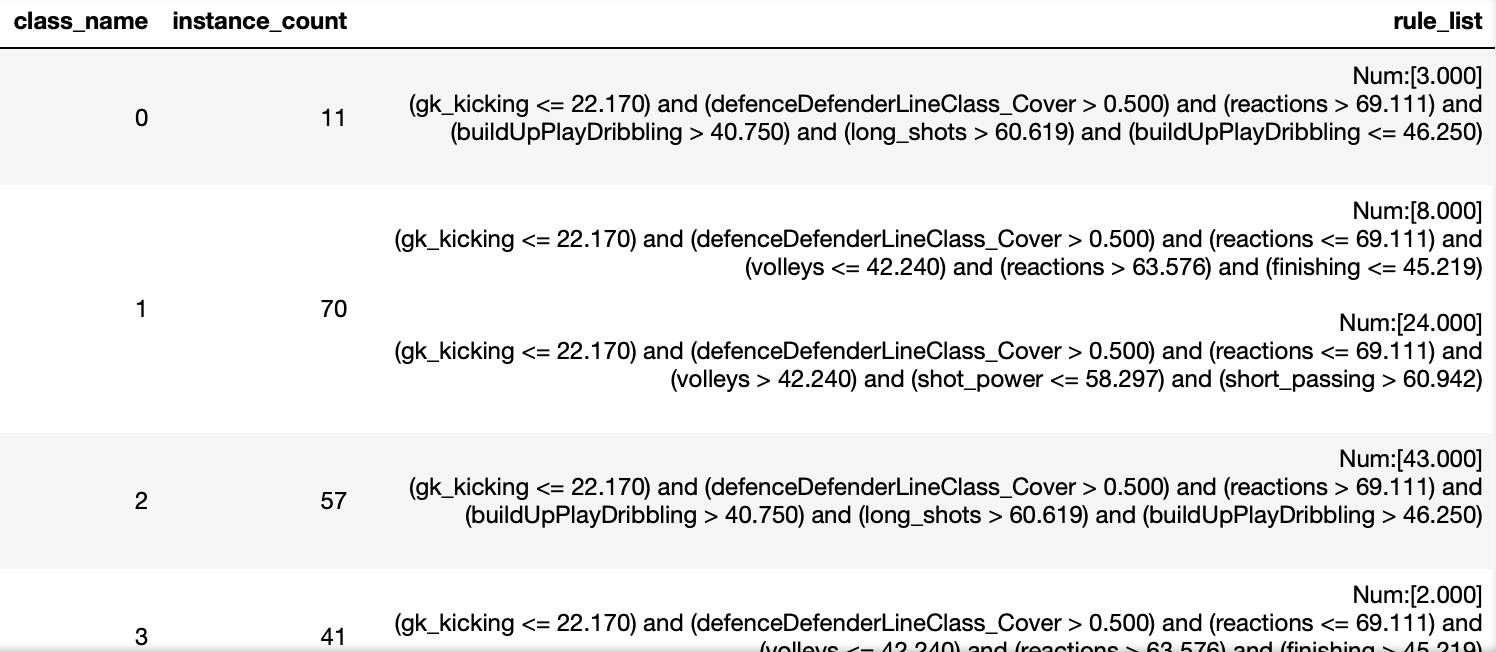
\includegraphics[width=.8\textwidth]{dc.png}
\caption{Generating rules for meta strategy assignment}
\label{fig:dc}
\end{figure}

Here we refer to Fig 8 on the expected number of goals by the best counter meta. 
\par Looking at the summary, a few features stand out. First of all, meta-strategy 9 leads all strategies in terms of average goals against other strategies, as well as having only itself as its most significant counter. On the other hand, we also witness chains of `dominance' such as
\[
    21 \to 5 \to 19 \to 17 \to 7 \to 23
\]
where the preceding strategy trumping the proceeding ones in the chain above. While our analysis only provides correlation and hence is limited in its ability to explain the causal factors behind such observations, we can make an attempt based on the learned categorization rules of our meta-strategies. 
\par In particular, we noted after running a decision tree categorization on the meta-strategies that strategy 9 leads all strategies in terms of the average overall rating and potential rating of its players. On the other hand, however, strategy 9 has average to low scores for team attributes such as dribbling and passing. This strategy, therefore, almost seem to present itself as an antithesis to the hypothesis that there exist meta-game strategies in soccer. We will look further into this issue in a later section. 
\par On the other hand, the identified chain of dominance is particularly interesting as we can identify defining traits of each meta-strategy that might explain some of the relationships. 
\par For instance, upon running a simple decision tree algorithm on the identified meta-strategies, we saw that strategy 21 can be defined by the high proportion of teams that adopt an \emph{offside trap} defensive maneuver. In soccer, the offside trap works by having a defensive line far up on the field, such that opposing strikers run the risk of getting fouled by rule of \emph{offside}. \footnote{In soccer, an offside foul is when an attacker is beyond the second last enemy player before a ball is passed to him} 
\par The offside trap is particularly effective against opponents who make medium to long range passes, which are then susceptible to having receivers be in an offside position. On the other hand, however, it can be countered by build up plays that heavily rely on dribbling. Incidentally, we saw that meta-strategy 5, which 21 dominates, can be identified by teams with \emph{Buildup Play Dribbling} of $< 40.8$ and \emph{Buildup Play Passing} of $> 46.5$. This suggests that teams which rely on passing up the field tend to suffer against teams of meta-strategy 21, just as our intuitive analysis indicates. 
\par Interestingly, however, we did not manage to identify any obvious (high deviation in win rate from 50-50) `cycles` of dominance. While chains of dominance do exist in most strategic games, in developed metagames it is often the case that only cycles survive eventually. For instance, a cycle would be a set of three meta-strategies that follow a `scissor-paper-stone' relationship. 
\par This is because in a strategic game, once identified, no team will adopt the lowest lying meta-strategy in a chain of dominance. This will in turn cause the second-lowest meta-strategy to be the weakest. Inductively, no team will adopt any strategy other than the top-level meta-strategy. Where there is a cycle, however, we will see a percentage of teams adopting every possible meta-strategy in the cycle. 
\par We unfortunately were unable to identify clear cycles in our meta-strategy clusters. However, we believe that this could be due to a structural limitation of soccer in the first place. Traditionally, in a strategic game, teams would change their play styles to adopt the most effective meta-strategies available. This assumes however that this change of play styles is quick to implement and will be as effective as the masters of the particular play style. This is simply not the case in soccer. Soccer teams are limited by player contracts, so they cannot switch out players with ease. They are also limited by the fact that it takes time, team cohesion and coaching knowledge to adopt new play styles on the fly. As a result, the soccer meta did not evolve as expected.

\subsection{Limitations}
Due to limited time and resources, we are aware of various weaknesses of our approach. 
\par In calculating player attributes, we took the aggregated mean over matches for each team. While this is a convenient way of integrating player attributes into each team, this ignores the fact that different features have different impacts on distinct roles. For instance, defensive ratings might not apply as much for strikers, while offensive ratings might not be as applicable for defenders. Goalkeeper ratings, on the other hand, are almost irrelevant to field players. 
\par Furthermore, the biggest question mark on our results is the existence of meta-strategy 9. This is the most dominant strategy cluster, with only itself as the sole reliable counter, but it turns out from looking deeper that the great identifying feature is the pure over skill rating of the team's players. Rather than disproving our `meta-game' hypothesis of football leagues, however, it is not unreasonable to expect that with sufficiently strong players, certain strategic disadvantages can be neutralized. Furthermore, attribute information might suffer from bias as they could be affected by team play style in the first place. Indeed, teams with an innately aggressive and fast play style could allow players to demonstrate higher levels of acceleration, for example. Teams that relied on set pieces could have strategies that relied on mid-ranged passing and drawing opposition attention. These are examples of hidden attributes that produce the given attributes as a consequence, instead of the other way round. Our models make use of the given attributes as a starting point, and as such might be limited in identify these hidden structures. 

\section{Conclusion}
In conclusion, through the datasets we have shown that we can identify distinct meta-strategies. As validation, we identified certain characteristics in our meta-strategy table that has reasonable real-life justifications. We did make various simplifying assumptions that might have limited the usefulness of our results; for instance, the fact that a meta-strategy that simply identify teams with `the best players' in meta-strategy 9 does not seem useful in identifying team playstyles. 
\par With more time and resources, we see great potential in removing such anomalies. We could possibly model each meta-strategy's win rate as a base rate scaled by the average rating of the team's players. This will take into account the fact that a team with stronger players might be able to neutralize meta-strategic disadvantages. 
\par Furthermore, we mentioned under limitations that the given attributes could be secondary features that arise from hidden attributes of meta-game strategies. To explore this issue, we could make use of neural nets in a manner which allows us to identify hidden structures behind the player attributes.  

\clearpage

\begin{thebibliography}{99} % Bibliography - this is intentionally simple in this template

\bibitem{1}“The Evolution of Barcelona's Tiki Taka.” The Evolution of Barcelona's Tiki Taka | Goal.com, www.goal.com/en/news/12/spanish-football/2015/09/29/15804882/the-evolution-of-barcelonas-tiki-taka. 

\bibitem{2}“The Evolution of Barcelona's Tiki Taka.” The Evolution of Barcelona's Tiki Taka | Goal.com, www.goal.com/en/news/12/spanish-football/2015/09/29/15804882/the-evolution-of-barcelonas-tiki-taka. 

\bibitem{3}Desmond, Rhys. “Counter Attacking and the Death of Tiki-Taka Football.” The MastermindSite, 7 Feb. 2021, themastermindsite.com/2019/09/21/counter-attacking-and-the-death-of-tiki-taka-football/. 

\end{thebibliography}

\end{document}
